\documentclass[11pt]{article}
\usepackage[pdftex]{graphicx}
\usepackage{html}
\usepackage{psfig}
\usepackage{makeidx}
\usepackage{nomencl}
\usepackage{tabularx}
\usepackage[letterpaper, top=1.0in, bottom=1in, inner=1.0in, outer=1.0in, foot=.25in]{geometry}

\newif\ifpdf\ifx\pdfoutput\undefined\pdffalse\else\pdfoutput=1\pdftrue\fi
\newcommand{\pdfgraphics}{\ifpdf\DeclareGraphicsExtensions{.pdf,.jpg}\else\fi}

\oddsidemargin  -0.1in   %  Note that \oddsidemargin = \evensidemargin
\evensidemargin -0.1in


%\topmargin -55pt         %    Nominal distance from top of page to top
%                         %    of box containing running head.
%\headheight 12pt         %    Height of box containing running head.
%\headsep 25pt            %    Space between running head and text.
%\footskip 60pt           %    Distance from baseline of box containing


%\textheight 9.125in        % Height of text (including footnotes and
                         % figures, excluding running head and foot).
%\textwidth 6.75in         % Width of text line.
                         % For two-column mode:

%\textheight 9.125in        % Height of text (including footnotes and
                         % figures, excluding running head and foot).
%\textwidth 6.75in         % Width of text line.
                         % For two-column mode:
\renewcommand{\baselinestretch}{1.2}
\renewcommand{\nomname}{Glossary}
\makeindex\makeglossary


\newcounter{sqlquerycounter}
\setcounter{sqlquerycounter}{1}
\newcommand{\sqlquery}[1]{
{\renewcommand\baselinestretch{.8}\rm
\begin{samepage}
\setlength{\parskip}{.1\baselineskip} 
\small
\hspace{.3in}\parbox[t]{5in}{\setlength{\parindent}{-.1in}\tt{#1}\\}
\normalsize
\renewcommand\baselinestretch{1.0}\rm
%\vspace{-22pt}
\end{samepage}
}}

\newcounter{lastquery}
\newcommand{\numsqlquery}[1]{
(\thesqlquerycounter) \sqlquery{#1}
\setcounter{lastquery}{\value{sqlquerycounter}}
\refstepcounter{sqlquerycounter}
}
\newcommand{\queryref}[1]{
\newcounter{#1}
\setcounter{#1}{\value{lastquery}}
}

\newcommand{\docroot}{tinyos-1.x}       
\newcommand{\java}{tinyos-1.x/tools/java}

\begin{latexonly}
\title{\vspace{2.5in} TinyDB:  In-Network Query Processing in TinyOS}
\end{latexonly}
\begin{htmlonly}
\title{TinyDB:  In-Network Query Processing in TinyOS}
\end{htmlonly}
\author{Sam Madden, Joe Hellerstein, and Wei Hong \\
        \{madden,jmh\}@cs.berkeley.edu, whong@intel-research.net}
\date{}

\begin{document}
\pdfgraphics
\pagenumbering{arabic}
%\pagestyle{myheadings}
\markright{{\bf TinyDB\index{TinyDB} Documentation. }}

\maketitle
\begin{latexonly}
\vspace{2in}
\end{latexonly}
\begin{center}
Version 0.4 \\
September, 2003
\end{center}


\thispagestyle{empty}
\begin{latexonly}\newpage\end{latexonly}
\tableofcontents
\begin{latexonly}\newpage\end{latexonly}

\section{What's New In This Release}

This document refers to the TinyDB 1.1 release, which 
accompanied TinyOS 1.1 and was officially released September, 2003
and represents major changes to the functionality and stability
of TinyDB, particularly over the 1.0 release.

For users already familiar with TinyDB, new features in this release
include:

\begin{itemize}
  
\item {\bf Queries over Flash Memory}: Queries in TinyDB can now log
  to the on-mote Flash, via the Matchbox filing system.  Logged query
  results can be read fetched via queries as well.  See Section
  \ref{sec:flash} for syntax and usage details.
  
\item {\bf Support for New Sensor-Boards and Sensors}: TinyDB supports
  the new Mica2 and Mica2Dot motes as well as a variety of new sensors
  for detecting air-pressure, humiditity, temperature and light.  It
  also includes code to calibrate these readings on the PC after they
  have been retrieved.  See Section \ref{sec:sb-config}.
  
\item {\bf New, Modularized Network Interface}: The network interfaced
  used by TinyDB has been totally rewritten.  The default interface
  improves multi-hop routing stability, and it is now much easier to
  replace the default routing with new routing layers that provide
  alternative functionality.  Section \ref{sec:tinydbnetwork} has been
  rewritten to reflect these changes.
  
\item {\bf New, Modularized Aggregate Interface}: It is now much
  easier to extend TinyDB with new aggregate operators. Section
  \ref{sec:adding-aggs} gives a brief tutorial on this.
  
\item {\bf Power Management}:When running queries with long sample
  periods, TinyDB intelligently power consumption, allowing the
  network to last for months a time.  Sections \ref{sec:time-sync} and
  \ref{sec:pm-config} describe these features.
  
\item {\bf Time Synchronization}: Sensors in TinyDB are now time
  synchronized.  This means that aggregate results are guaranteed to
  have been collected at the same time, and that motes agree on the
  real-world start and end-time of every epoch. Section
  \ref{sec:time-sync} also includes details about these features.
  
\item {\bf Event-based Queries}: TinyDB includes support for queries
  that are initiated by low-level operating system ``events''.  These
  events can be defined much like commands and attributes, and
  referenced in queries.  See Section \ref{sec:event-queries} for more
  details.
  
\item {\bf Tiny Application Sensor Kit (TASK)}: TinyDB is at the core of the
  new ``tiny application sensor kit'', a toolkit that provides a new
  user-interface and relational database interface for collecting data
  from TinyDB.  Section \ref{sec:task} summarizes the kit and provides
  pointers to documentation.

\item {\bf Simulator Support}: TinyDB now runs in the TOSSIM simulator, which can
  be useful for debugging or demonstration purposes.  Section \ref{sec:tossim}
  describe running TinyDB in the simulator.
  
\item {\bf New Debugging, Testing, and Status Tools}: Finally, several
  new tools and interfaces have been added to make it much easier to
  retrieve status information from TinyDB and listen to TinyDB
  specific network traffic. Section \ref{sec:debugging} describes these features.

\end{itemize}

\section{Introduction}

TinyDB\index{TinyDB} is a query processing system for extracting
information from a network of
\htmladdnormallink{TinyOS}{http://webs.cs.berkeley.edu/tos}
sensors.\index{TinyOS}\index{sensor} Unlike existing solutions for
data processing in TinyOS\index{TinyOS}, TinyDB\index{TinyDB} does not
require you to write embedded C\index{C} code for
sensors\index{sensor}\index{embedded}.  Instead, TinyDB\index{TinyDB}
provides a simple, SQL\index{SQL}-like interface to specify the data
you want to extract, along with additional parameters, like the rate
at which data should be refreshed -- much as you would pose queries
against a traditional database.  Given a query specifying your data
interests, TinyDB\index{TinyDB} collects that data from
motes\index{mote} in the environment, filter\index{filter}s it,
aggregates\index{aggregate} it together, and routes\index{routing} it
out to a PC.  TinyDB\index{TinyDB} does this via power-efficient
in-network\index{in-network} processing algorithms.

To use TinyDB\index{TinyDB}, you install its TinyOS\index{TinyOS} components\index{component} onto
each mote\index{mote} in your sensor\index{sensor} network. 
%(TinyDB\index{TinyDB}'s components\index{component} can co-exist
%with other components\index{component}, although they can place extensive demands on
%the memory and radio resources of the mote\index{mote}.)  
TinyDB\index{TinyDB} provides a simple Java\index{Java} API\index{API}
for writing PC applications that query and extract data from the
network; it also comes with a simple graphical query-builder and
result display that uses the API\index{API}.

The primary goal of TinyDB\index{TinyDB} is to make your life as a programmer
significantly easier, and allow data-driven applications to be
developed and deployed {\em much} more quickly than what is currently
possible.  TinyDB\index{TinyDB} frees you from the burden of writing low-level code
for sensor\index{sensor} devices, including the (very tricky) sensor network\index{sensor network}
interfaces.  Some of the features of TinyDB\index{TinyDB} include:

\begin{itemize}
\item {\it Metadata Management\index{catalog}}: TinyDB provides a
  metadata catalog to describe the kinds of sensor readings that are
  available in the sensor network.
\item {\it High Level Queries}: TinyDB uses a {\em
    declarative}\index{declarative} query language that lets you
  describe the data you want, without requiring you to say how to get
  it.  This makes it easier for you to write applications, and helps
  guarantee that your applications continue to run efficiently as the
  sensor network changes.
\item {\it Network Topology\index{topology}}: TinyDB\index{TinyDB}
  manages the underlying radio network by tracking
  neighbors\index{neighbor}, maintaining routing\index{routing}
  tables, and ensuring that every mote\index{mote} in the network can
  efficiently and (relatively) reliably deliver its data to the user.
\item {\it Multiple Queries}: TinyDB\index{TinyDB} allows multiple
  queries to be run on the same set of motes\index{mote} at the same
  time.  Queries can have different sample\index{sample} rates and
  access different sensor\index{sensor} types, and
  TinyDB\index{TinyDB} efficiently shares work between queries when
  possible.
\item {\it Incremental Deployment via Query Sharing}: To expand your
  TinyDB\index{TinyDB} sensor network\index{sensor network}, you
  simply download\index{download} the standard TinyDB\index{TinyDB}
  code to new motes\index{mote}, and TinyDB\index{TinyDB} does the
  rest.  TinyDB\index{TinyDB} motes\index{mote} share queries with
  each other: when a mote\index{mote} hears a network message for a
  query that it is not yet running, it automatically asks the sender
  of that data for a copy of the query, and begins running it.  No
  programming or configuration of the new motes\index{mote} is
  required beyond installing TinyDB\index{TinyDB}.
\end{itemize}

This document serves a number of purposes.  The first sections are
targeted at the sensor\index{sensor} application programmer, and include a basic
overview of the TinyDB\index{TinyDB} system architecture, and a QuickStart guide to
using the TinyDB\index{TinyDB} system, its query language and APIs\index{API}.  The remaining
sections are targeted at readers who want to extend the TinyDB\index{TinyDB} system
itself.
%%  We never added this stuff.
%   They describe the TinyDB\index{TinyDB} software components\index{component}, highlighting
% places where the system could be profitably extended.

\subsection{System Overview}

This section provides a high level overview of the architecture of the
TinyDB\index{TinyDB} software.  It is designed to be accessible to
users of the TinyDB\index{TinyDB} system who are not interested in the
technical details of the system's implementation.  A detailed
description of the TinyDB\index{TinyDB} software design is reserved
for Sections~\ref{sec:devel} and~\ref{sec:inside}.

We begin with a short description of a typical use-case for TinyDB\index{TinyDB}.  Imagine that Mary
wishes to locate an unused conference room in her sensor\index{sensor}-equipped building, and
that an application to perform this task has not already been built.
The motes\index{mote} in Mary's
building have a sensor board\index{sensor board} with light sensors\index{sensor} and microphones and have been programmed with
a room number.  Mary decides that her application
should declare a room {\it in-use} when the average light reading of all the sensors\index{sensor} in a room
are above $l$ and when the average volume is above $v$.  Mary wants her application to 
refresh this occupancy information every 5 minutes.  Without TinyDB\index{TinyDB}, Mary
would have to write several hundred lines of custom embedded C\index{C}
code~\index{embedded} to collect information
from all the motes\index{mote} in a room, coordinate the communication of readings
across sensors\index{sensor},
aggregate\index{aggregate} these readings together to compute the average light
and volume, and then forward that information from within the sensor network\index{sensor network} to the PC where
the application is running.  She would then have to download\index{download} her compiled\index{compile}
program to each of the motes\index{mote} in the room.  Instead, if the motes\index{mote} in Mary's building are running TinyDB\index{TinyDB},
she can simply pose the following SQL\index{SQL}
query to identify the rooms that are currently in-use:

\noindent{\tt \hspace{.5in}SELECT\index{Select} roomno, AVG(light), AVG(volume) \\
\hspace*{.5in}FROM\index{From} sensors\index{sensor} \\
\hspace*{.5in}GROUP BY\index{Group By}\index{group} roomno \\
\hspace*{.5in}HAVING\index{Having} AVG(light) > $l$ AND AVG(volume) > $v$ \\
\hspace*{.5in}EPOCH DURATION\index{Epoch Duration} 5min
}

\noindent TinyDB\index{TinyDB} translates this query into an efficient
execution plan\index{query plan} which
delivers the set of occupied rooms every 5 minutes\index{epoch}.  Mary simply inputs this query
into a GUI\index{GUI} -- she writes no C\index{C} code and is freed from 
concerns about how to install her code, how to propagate results across
multiple network hops\index{hop}\index{multi-hop} to the root\index{root} of the network, how to power down sensors\index{sensor} 
during the time when they are not collecting and reporting data, and many other
difficulties associated with sensor-network\index{sensor network} programming.

We discuss the inner workings of TinyDB\index{TinyDB} on such queries in
Sections~\ref{sec:devel} and~\ref{sec:inside} below.  In the remainder of this section, we
present a high-level overview of the components\index{component} of TinyDB\index{TinyDB}.  The system
can be broadly classified into two subsystems:

\begin{enumerate}
\item \underline{Sensor Network\index{sensor network} Software:}  This is the heart of TinyDB\index{TinyDB}, although most users of
the system should never have to modify this code.  It runs on each
mote\index{mote} in the network, and consists of several major pieces:
\begin{itemize}
\item {\it Sensor\index{sensor} Catalog\index{catalog} and Schema\index{schema} Manager}:  The catalog\index{catalog} is responsible for tracking the
set of {\it attributes\index{attribute}}, or types of readings
(e.g.\ light, sound, voltage) and
properties (e.g.\ network parent\index{parent}, node\index{node} ID\index{ID}) available
on each sensor\index{sensor}.  In general, this list is not identical for each sensor\index{sensor}:  networks may consist
of heterogeneous collections of devices, and may be able to report
different properties.  (See
Section~\ref{sec:catalog} for details.)

\item {\it Query Processor\index{query processor}}: The main
component\index{component} of TinyDB\index{TinyDB} consists of a small
query processor\index{query processor}.  The query
processor\index{query processor} uses the catalog\index{catalog} the
fetch the values of local attributes\index{attribute}, receives
sensor\index{sensor} readings from neighboring\index{neighbor}
nodes\index{node} over the radio, combines and
aggregates\index{aggregate} these values together,
filters\index{filter} out undesired data, and outputs values to
parent\index{parent}s.  (See Section~\ref{sec:qp} for details.)

\item {\it Memory Manager}:  TinyDB\index{TinyDB} extends TinyOS\index{TinyOS} with a small, handle-based\index{handle}
  dynamic memory manager.  (See Section~\ref{sec:tinyalloc} for details.)

\item {\it Network Topology\index{topology} Manager}: TinyDB\index{TinyDB} manages the connectivity
  of motes\index{mote} in the network, to efficiently
  route\index{routing} data and query 
  sub-results through the network.  (See Section~\ref{sec:tinydbnetwork}
  for details.)
\end{itemize}
\item \underline{Java\index{Java}-based Client\index{client} Interface:}
A network of TinyDB\index{TinyDB} motes\index{mote} is accessed from a connected PC through the
{\em TinyDB\index{TinyDB} client\index{client} interface}, which consists
of a set of Java\index{Java} classes and applications.  These classes are all stored in the {\tt {\java}/tinyos/tinydb} 
package in the source tree.  The specific classes are described in Section \ref{sec:devel};  major
classes include:
\begin{itemize}
\item A network interface class that allows applications to inject queries and listen for results (Section~\ref{sec:tinydbnet}) 
\item Classes to build and transmit queries (Sections~\ref{sec:tinydbquery}, \ref{sec:tinydbaggop}, \ref{sec:tinydbselop})
\item A class to receive and parse query results (Section~\ref{sec:tinydbqueryresult})
\item A class to extract information about the attributes\index{attribute} and capabilities of devices (Section~\ref{sec:tinydbcatalog})
\item A GUI\index{GUI} to construct queries (Sections~\ref{sec:queryframe}, \ref{sec:queryfield})
\item A graph and table GUI\index{GUI} to display individual sensor\index{sensor} results (Sections~\ref{sec:resultframe}, \ref{sec:resultgraph}, \ref{sec:plot})
\item A GUI\index{GUI} to visualize dynamic network topologies (Section~\ref{sec:topology})
\item An application that uses queries as an interface on top of a network of sensors (Section~\ref{sec:app})\index{sensor}
\end{itemize}
\end{enumerate}

\section{Quick Start:  Running Queries with TinyDB\index{TinyDB}} \label{sec:runningqueries}

In this section, you will learn how to install TinyDB software, set up a network of TinyDB\index{TinyDB} motes\index{mote}, inject a query
into the network, and collect the results of the query.  

\subsection{Installation and Requirements}
TinyDB\index{TinyDB} requires a basic TinyOS\index{TinyOS} installation, with a working Java\index{Java}
installation (and javax.comm library).  
%For installation instructions
%on TinyOS\index{TinyOS}, see the \htmladdnormallink{TinyOS\index{TinyOS} web
%page}{http://webs.cs.berkeley.edu/tos}.
It is currently designed to work with the nesC compiler (next generation C-like language for TinyOS) 
and avr-gcc 3.3 \index{avr-gcc}\index{gcc}.  To obtain these tools, download the 
TinyOS 1.1 release from 

\htmladdnormallink{http://webs.cs.berkeley.edu/tos}{http://webs.cs.berkeley.edu/tos}

Click on the link for your platform (PC Linux or Windows), and
follow the installation instructions.

The most recent version of TinyDB is always available from the TinyOS SourceForge
repository;
%TinyDB\index{TinyDB} is not currently a part of an official TinyOS\index{TinyOS} release.  To obtain
%the code, you will need to check out a recent version of TinyOS from CVS;  
see the
\htmladdnormallink{TinyOS\index{TinyOS} CVS Page}{http://sf.net/cvs/?group_id=28656}
for instructions on using CVS.
In addition to the standard TinyOS\index{TinyOS} distribution, TinyDB includes a number of
additional files detailed in Appendix~\ref{app:files} of this document. The following table summarizes the software requirements of TinyDB: 

\par
\tiny
\begin{tabular}{|l|l|}
\hline
Required Software & Notes \\
\hline\hline
avr-gcc \index{avr-gcc}\index{gcc} & Version 3.3 or later \\ 
Java SDK \index{Java} & Version 1.4 or later \\
nesC compiler \index{nesC} & From the TinyOS 1.1 release \\
javax.comm tools & Version 1.3 or later, from IBM \\
TinyOS & From SourceForge CVS \\
\hline
\end{tabular}
\normalsize
\\

\noindent To verify that your installation is working properly, do the following:

\begin{enumerate}
\item Compile\index{compile} and install TinyDB\index{TinyDB} on the mote\index{mote}.  To do this, connect the mote\index{mote} to
the programming board\index{programming board}, then type the following:
\begin{itemize}
\item {\tt cd \docroot/apps/TinyDBApp/}
\item {\tt make mica}
\item {\tt make mica install}
\end{itemize}
If this fails, verify that your installation works (see the instructions on the web
site), and that you have all of the TinyDB\index{TinyDB} files listed above.

\item Compile\index{compile} and run the TinyDB\index{TinyDB}Main java\index{Java} classes.  To do this, type the following:
\begin{itemize}
\item {\tt cd {\java}/net/tinyos/tinydb}
\item {\tt make}
\item {\tt cd {\java}}
\item {\tt java net.tinyos.tinydb.TinyDBMain}
\end{itemize}

You'll need to make sure you have the following jar files in your classpath (they should all be available in {\tt {\java}/jars}):
\begin{itemize}
\item {\tt JLex.jar}
\item {\tt cup.jar}
\item {\tt plot.jar}
\item {\tt xercesImpl.jar}
\item {\tt xmlParserAPIs.jar}
\end{itemize}

You must also have the {\tt {\java}} directory in your classpath.  


If you wish to take advantage of TinyDB's compatibility with the PostgreSQL\index{PostgreSQL} 
database system, you'll need 
to install and configure Postgres (see Section \ref{postgres}) 
 and include the {\tt pgjdbc2.jar} file in your classpath.

Your {\tt CLASSPATH} should now look something like this:

{\tt
.:{\it /path/to/java}/jre/lib/rt.jar:{\it /path/to/java}/lib/dt.jar:\\
{\it /path/to/java/}lib/tools.jar:/opt/IBMJava2-13/jre/lib/ext/comm.jar:\\
{\java}/jars/plot.jar:{\java}/jars/cup.jar:\\
{\java}/jars/xercesImpl.jar:{\java}/jars/xmlParserAPIs.jar:\\
{\java}/jars/JLex.jar:{\java}
}

If you installed TinyOS and TinyDB
from the TinyOS 1.1 RPMS, your classpath should have been automatically configured to include these
files (as well as a number of files, which should not be a problem.)

\end{enumerate}


\noindent You may see warnings about ``deprecated classes'' when {\tt
javac}\index{javac} runs.  These are OK, and you can ignore them.  After running
the java\index{Java} command, you should see the TinyDB\index{TinyDB} control
panel and query interface appear.

Once you have a working installation of these files, continue on to the next section
to learn how to run queries with TinyDB\index{TinyDB}.

\subsection{Setting up a Network of TinyDB\index{TinyDB} motes\index{mote}}

The first step is to program a number
of motes\index{mote} with the TinyDB\index{TinyDB} software.  Each of these motes\index{mote} must have a unique ID\index{ID};  recall that,
in TinyOS\index{TinyOS}, you can set the ID of a mote\index{mote} when running {\tt make install} by appending {\tt .node\index{node}id}
-- for example, to program a TinyDB\index{TinyDB} mote\index{mote} at ID 2, you would type:

\begin{itemize}
\item {\tt cd \docroot/apps/TinyDBApp/}
\item {\tt make mica install.2}
\end{itemize}

\noindent To run TinyDB\index{TinyDB}, you will need at least two
motes\index{mote}: one to act as the basestation
mote\index{basestation}, and one or more to distribute and run queries
over.  You may want to place a sticker on your chosen basestation
mote, since you will need to identify it visually. All
motes\index{mote}, including the basestation\index{basestation}, run
the same {\tt TinyDBApp} application, however, {\it the
basestation\index{basestation} mote\index{mote} must be set to ID\index{ID} 0.}

After programming your motes\index{mote}, connect the programming
board\index{programming board} to your computer via the serial
port\index{serial}, and place the basestation\index{basestation} mote\index{mote} in the programming
board\index{programming board}.  Turn on all of the motes\index{mote}.

Figure \ref{fig:setup} illustrates the basic setup of motes and PC.  

\begin{figure}[h]
\centering\leavevmode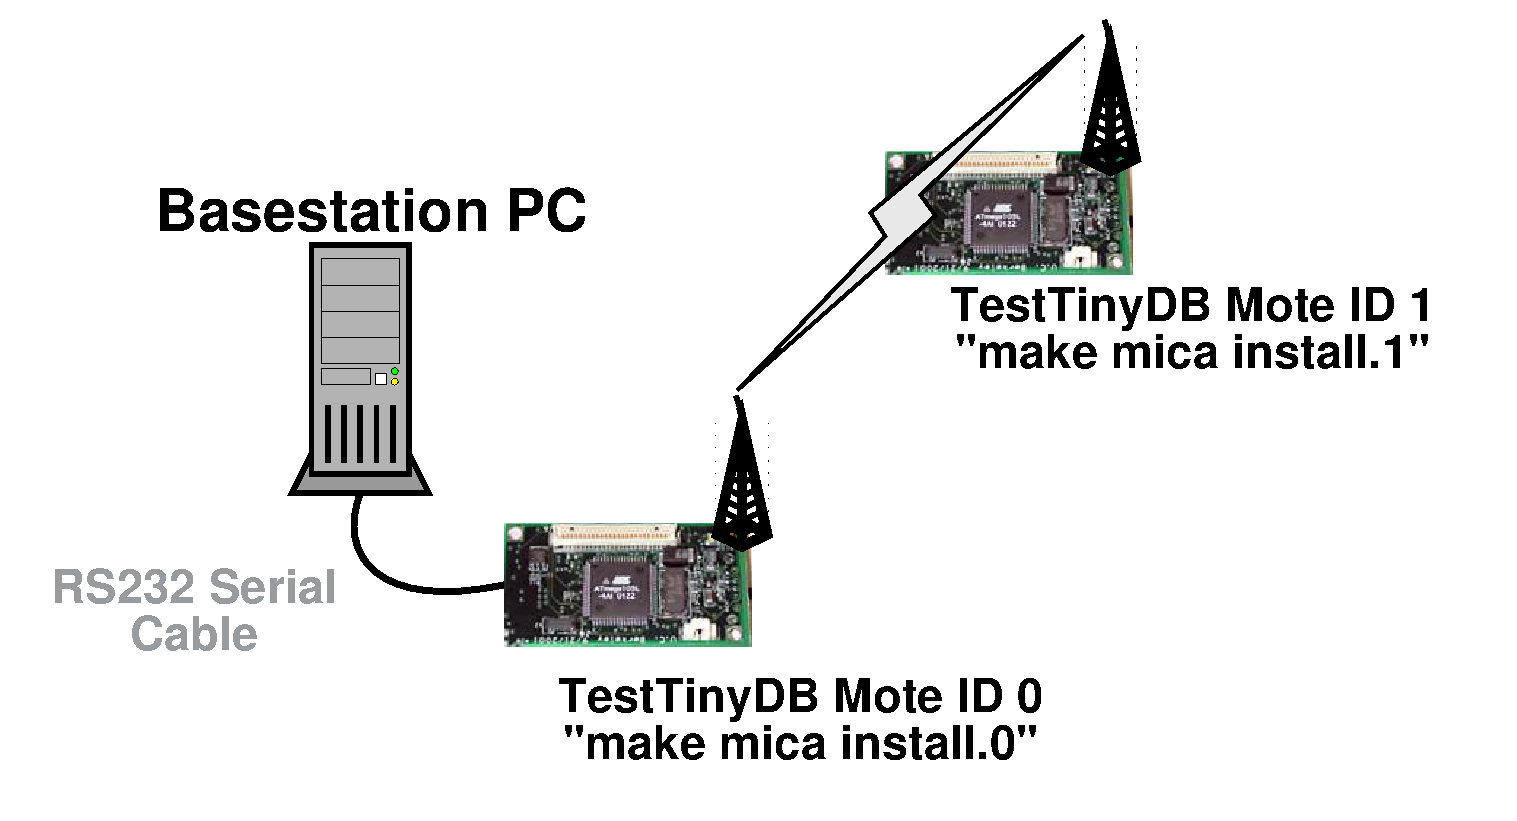
\includegraphics[width=3in]{setup}
\caption{Two TinyDB motes set up to run a query.}
\label{fig:setup}
\end{figure}


\subsection{Running the TinyDB\index{TinyDB}Main GUI\index{GUI}}
\label{sec:GUI}
The TinyDB\index{TinyDB}Main Java\index{Java} application provides a graphical interface for distributing queries 
over motes\index{mote} and collecting data from them.  To run this application, type:

\begin{itemize}
\item {\tt cd {\java}/net/tinyos/tinydb}
\item {\tt make}
\item {\tt cd {\java}}
\item {\tt java net.tinyos.tinydb.TinyDBMain}
\end{itemize}

Two windows should appear; one, the {\it command}\index{command} window (Figure
\ref{fig:command}), allows you to send a variety of control commands
to the motes\index{mote}.  The other, the {\it query} window (Figure
\ref{fig:query}), allows you to build and send queries into the
network.  We will be focusing on the operation of the query window in
the next section; the command window is fairly self-explanatory.

The query window contains a {\bf Display Topology} button to show the
network topology. This button actually generates a particular query
that is executed by the motes, with results displayed in a special
visualization.  It is a good idea to display you network topology and
make sure that all your motes are alive and communicating.

Once you see that your network of motes is operational, you can
proceed to constructing queries.  

\vspace{.1in}
\renewcommand{\baselinestretch}{1.0}\rm
\fbox{\parbox{.9\columnwidth}{
{\bf TIP:} If you have difficulty sending queries
into the network, verify that the {\tt comm-string}
in {\tt \java/tinydb.conf} has been set correctly;
see Section \ref{sec:configfile} for more information.
A common problem is the wrong setting of the UART baud rate.
The correct baud rates are 19200 for mica and mica2dot,
57600 for mica2.}}
\renewcommand{\baselinestretch}{1.2}\rm

\begin{figure}
\begin{minipage}{4in}
\begin{center}
\leavevmode
{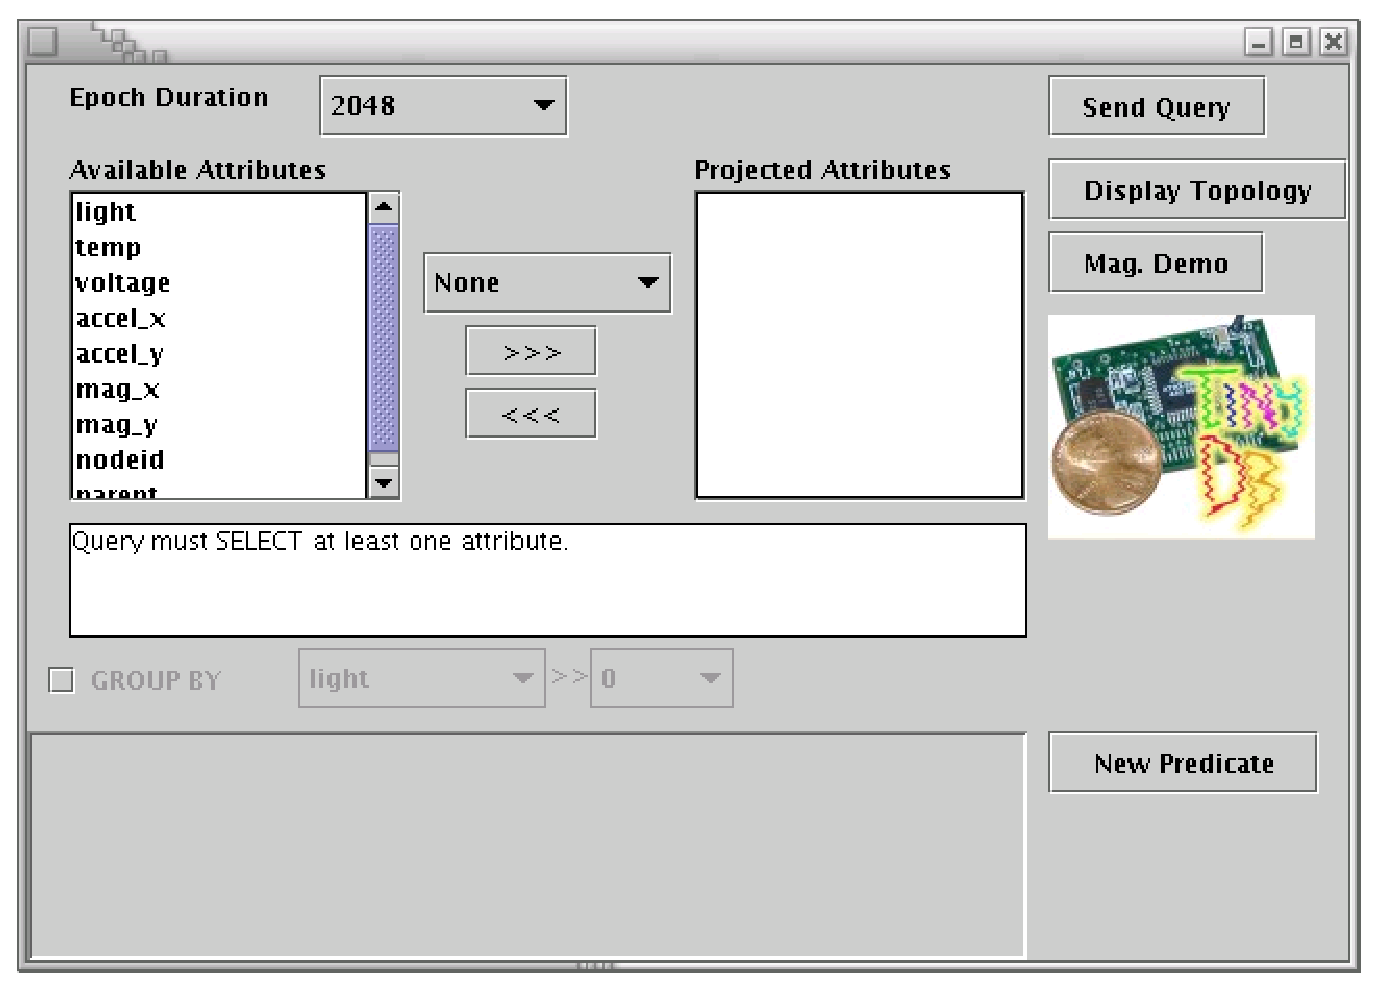
\includegraphics[width=3in]{querywin}}
\end{center}
\caption{Query Window}
\label{fig:query}

\end{minipage}
\hspace{.5in}
\begin{minipage}{2in}
\begin{center}
\leavevmode
{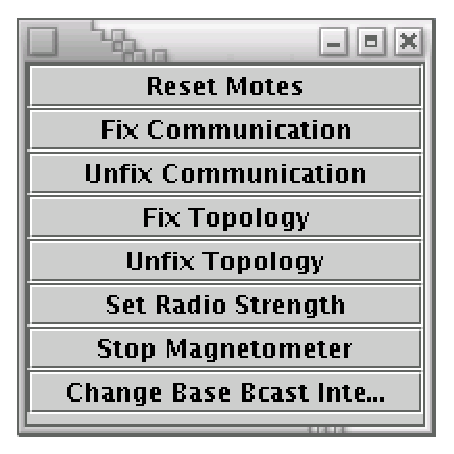
\includegraphics[width=1.5in]{commandwin}}
\end{center}
\caption{Command Window}
\label{fig:command}
\end{minipage}
\end{figure}

\section{Using TinyDB\index{TinyDB}}
\label{sec:queries}
TinyDB provides a high-level, {\em declarative}\index{declarative}
language for specifying queries.  In a declarative language you
describe {\em what} you want, but not {\em how} to get it.
Declarative languages are advantageous for two reasons.  First, they
are relatively easy to learn, with queries that are easy to read and
understand.  Second, they allow the underlying system to change how it
runs a query, without requiring the query itself to be changed.  This
is important in a volatile context like sensor networks, where the
best underlying implementation may need to change frequently --
e.g. when motes move, join or leave the network, or experience
shifting radio interference.  In TinyDB, the execution strategy for a
user query can change each time the query is run, or even {\em while}
the query runs, without any need for re-typing the query or
recompiling an application that embeds the query.

Before describing TinyDB's query facilities, a few words on
TinyDB's data model are in order.  TinyDB implicitly queries one
single, infinitely-long logical table\index{table} called {\tt sensors}.  This
table has one column for each attribute in the catalog\index{catalog}, including
sensor attributes, nodeIDs\index{ID}, and some additional ``introspective''\index{introspection}
attributes (properties) that describe a mote's state.  This table conceptually
contains one row for each reading generated by any mote, and hence the
table can be thought of streaming infinitely over time.  A given mote
may not be able to generate all the attributes, e.g., if it does not
have the sensor that generates the attribute.  In that case, the mote
will always generate a NULL value for that attribute.

TinyDB's query language is based on SQL\index{SQL}, and we will refer
to it as TinySQL\index{TinySQL}.  As in SQL, queries in
TinySQL\index{TinySQL} consist of a set of
attributes\index{attribute} to select (e.g. light, temperature), a set
of {\it aggregation\index{aggregation} expressions\index{expression}}
for forming aggregate result columns, a set of {\it
selection\index{selection} predicates\index{predicate}} for filtering\index{filter}
rows, and optionally a grouping\index{group} expression for
partitioning the data before aggregation.  Aggregation
is commonly used in the sensor environment.  

Currently, TinySQL\index{TinySQL} results are very similar to SQL\index{SQL}, in that they
are based on snapshots\index{snapshot} in time -- that is, they are
posed over rows generated by multiple sensors\index{sensor} at one
point in time.  {\it Temporal}\index{temporal} queries that combine
readings over several time periods are not supported in the current
release.  Instead, TinySQL runs each query repeatedly, once per
time-period or ``epoch''\index{epoch}.  The duration of an epoch can be specified
as part of a TinySQL query; the longer the duration, the less
frequent the results, and the less drain on the mote\index{mote} batteries\index{battery}.


\subsection{The Query Window}
\label{sec:querywindow}
The query window provides a graphical interface for building queries.
As you use the widgets in the window, query text is dynamically
constructed in the text box in the middle of the screen.  This box is
also used for error messages.

\vspace{.1in}
\renewcommand{\baselinestretch}{1.0}\rm
\fbox{\parbox{.9\columnwidth}{
{\bf TIP:}The current query text can
always be refreshed by clicking on a column in the {\bf Available
Attributes} list.}}
\renewcommand{\baselinestretch}{1.2}\rm
\vspace{.1in}

The topmost widget in the window is the {\bf Epoch
  Duration}\index{Epoch Duration}\index{epoch} widget,
which specifies the interval at which the query is re-evaluated.
% Motes periodically take sensor readings from the environment, called
% {\em samples}\index{sample}, in order to generate rows in the {\tt
% sensors} table.  
We recommend that the epoch duration be set as large as possible to
minimize power drain on the motes\index{mote}.

To specify the query to run each epoch\index{epoch}, you first choose the
attributes and/or aggregate expressions\index{expression} to appear in the output.
Attributes are specified by choosing them in the {\bf Available
Attributes} list, and pressing the ``$>>>$'' button so that they
appear in the {\bf Projected Attributes} list.  Optionally, attributes
may be placed in simple {\em aggregate}\index{aggregate} {\em
expressions}\index{expression} by choosing an aggregate from the
pull-down menu in the middle of the screen (default: {\bf None}).  At
this stage, the Projected Attributes list must
contain either all aggregate expressions, or all attributes; a mixture
will result in an error message unless there is a GROUP BY\index{Group By}\index{group}
clause.  We will return to this point shortly.

To select only some of the rows to be considered in the query, you can
specify predicates\index{predicate} to filter\index{filter} the data,
via the {\bf New Predicate} button at the bottom of the screen.  All
the predicates you select will be implicitly ``AND''ed together.  ``OR'' is
not yet supported.

If you used aggregate expressions\index{expression} in your {\bf Projected
Attributes} list, you can also specify a GROUP BY\index{Group By}\index{group} column by
clicking on the {\bf GROUP BY} checkbox and selecting from the
pulldown menu.  The pulldown menu to the right of the GROUP BY column
is for right-shifting the (binary) value of the column before
grouping; each shift divides the value of the GROUP BY column by 2.
This has the effect of reducing the number of possible groups: the
more times you divide by 2, the fewer possible groups there can be.

After adding a GROUP BY\index{Group By}\index{group} column, you can now add it (unaggregated!) to
the {\bf Projected Attributes} by selecting it from the {\bf Available
Attributes} list and pressing the ``$>>>$'' button.  This is the only
way to mix aggregates and attributes in your query
output\footnote{Note that this restriction also exists in SQL\index{SQL}, and is
implicit in the meaning of aggregation.  The only non-aggregated
attributes that are meaningful in the SELECT list are attributes that
appear in the GROUP BY list.  As an example, consider a query
with {\em no} GROUP BY attributes.  It can only produce one output row
per epoch\index{epoch}, which contains aggregate values computed from all the
input rows.  It is not meaningful to ask for a raw attribute in the
output of such a query -- there can be multiple values for each
attribute in the input, so there is no well-specified unique value to
place in the single output column.  The same restriction applies in a
GROUP BY query, with the exception of the columns in the GROUP BY
expression\index{expression} -- these columns are guaranteed to have a
single unique value per group, and hence can appear alongside aggregate
expressions.}.

\subsubsection{Triggers}\label{sec:triggers}\index{triggers}

TinyDB includes a facility for simple {\it triggers}\index{triggers}, or queries
that execute some command when a result is produced.  Currently, triggers can be
executed only in response to some local sensor reading that satisfies the conditions
specified in the {\tt WHERE} clause of the query.  {\it Aggregate queries cannot
have triggers associated with them.}  Whenever a query result satisfies the
{\tt WHERE} clause of a query, the {\it trigger action}\index{trigger action} is executed.  This
action is a named command stored in the schema of the mote (see Section \ref{sec:schema}
for more information.)  

The current TinyDB interface includes simple trigger actions\index{trigger action} for blinking LEDs and
sounding the sounder \index{sounder} (the small speaker on the Mica sensor board.)  A trigger
action can be specified via the GUI by clicking the {\tt TRIGGER ACTION} checkbox and selecting the appropriate
action.  Other actions can be specified via the textual interface (see the next section) and the schema
API (described in Section \ref{sec:schema}.)  

As an example of what triggers can be used for, consider an application where the user wants to sound
an alarm whenever the temperature near a sensor goes above some threshold.  This can be accomplished
via the simple trigger query:

\noindent{\tt \hspace{.5in}SELECT temp\\
\hspace*{.5in}FROM sensors \\
\hspace*{.5in}WHERE temp > {\it thresh}\\
\hspace*{.5in}TRIGGER ACTION SetSnd(512) \\
\hspace*{.5in}EPOCH DURATION 512
}

\noindent The {\tt SetSnd} command sounds the sounder, and the value of 512 specfies a sound duration of
512 ms.



\subsection{Composing Your Own TinyDB Queries}
\label{sec:tinydbsqlsyntax}
When using TinyDB, it is also possible to write queries by
hand, either by using the ``Text Interface'' pane of the the GUI\index{GUI}
(which can be brought up by default by using the command-line \index{command-line} argument ``-text''), 
or via the {\tt SensorQueryer.translateQuery} API\index{API} call.  We assume here that
the reader has a familiarity with the basics of SQL\index{SQL}.  A number of
books and websites provide simple SQL tutorials.  No deep knowledge of
SQL is required to use TinyDB; the basics will do.  The simplest way
to learn TinySQL\index{TinySQL} is to use the graphical query
builder described in Section~\ref{sec:querywindow}.  However, we also
provide a simple, informal description of the syntax here.

TinyDB provides an SQL\index{SQL}-like query language, which is simplified in a
number of ways, but which also provides some new sensor-specific syntax.
TinySQL\index{TinySQL} queries all have the form:

\noindent{\tt \hspace{.5in}SELECT {\em select-list}\\
\hspace*{.5in}[FROM sensors] \\
\hspace*{.5in}WHERE {\em where-clause}\\
\hspace*{.5in}[GROUP BY {\em gb-list} \\
\hspace*{.5in}[HAVING {\em having-list}]]\\
\hspace*{.5in}[TRIGGER ACTION {\em command-name}[({\em param})]] \\
\hspace*{.5in}[EPOCH DURATION {\em integer}]

}
 
The {\tt SELECT}\index{Select}, {\tt WHERE}\index{Where}, {\tt GROUP
  BY}\index{Group By}\index{group} and {\tt HAVING}\index{Having} clauses
are very similar to the functionality of SQL\index{SQL}.
Arithmetic\index{arithmetic} expressions\index{expression} are
supported in each of these clauses.  As in standard SQL, the {\tt
GROUP BY}\index{Group By} clause is optional, and if {\tt GROUP BY} is
included the {\tt HAVING}\index{Having} clause may also be used optionally.

\subsection{TinySQL\index{TinySQL} vs. Standard SQL\index{SQL}}

\noindent
{\bf Limitations}
\begin{itemize}
\item The {\tt FROM}\index{From} clause must always list exactly one table\index{table},
entitled {\tt sensors}.  The {\tt FROM}\index{Having} clause is also optional.
\item In the current version the {\tt WHERE}\index{Where} and {\tt
    HAVING}\index{Having} clauses can contain only simple conjunctions
  over arithmetic\index{arithmetic} comparison operators.  There is no
  support for the Boolean operators {\tt OR}\index{Or} and {\tt
    NOT}\index{Not}, or string matching\index{string matching}
  comparisons (SQL's\index{SQL} {\tt LIKE}\index{Like} and {\tt
    SIMILAR}\index{Similar} constructs).
\item  There is currently no support for sub-{\tt SELECT}s\index{Select} (subqueries)\index{subquery}.
\item There is currently no support for column renaming
  (SQL's\index{SQL} {\tt AS}\index{As} construct) in the {\em
    gb-list}.
\item Arithmetic\index{arithmetic} expressions\index{expression} are
  currently limited to the form {\em column op constant}, where {\em
    op} is one of \{$+, -, *, /$\}.
\end{itemize}

\noindent
{\bf Sensor-Specific Features}\\

The {\tt TRIGGER ACTION} clause specifies an (optional) trigger
action\index{trigger action} that should be executed whenever a query
result is produced.  See Section \ref{sec:triggers} for more
information about triggers.  The command name must be a command
registered with the {\tt COMMAND} \index{command} component (see
Section \ref{sec:schema}.)  An optional integer parameter may be
passed to the command.

The time between epochs\index{epoch} is specified in the query via the
{\tt EPOCH DURATION}\index{Epoch Duration} clause.  The units for this
duration are specified in milliseconds.  If no epoch duration is
specified, a value of 1024 ms is used by default.

\subsection{The Command Line}\label{sec:commandline}
TinyDB provides a few simple command line \index{command line}
options, as follows:

\begin{itemize}
\item {\tt -text}: Start the GUI in the text panel.\index{GUI}
\item {\tt -gui}: Start the GUI in the graphical query input window (default.)
\item {\tt -cmdwindow}: Display the command window (overrides the
  config file (see Section \ref{sec:configfile}) setting.)
\item {\tt -configfile {\it filename}}: Loads the config file from
  {\it filename}.\index{configuration}
\item {\tt -run ``{\it query}'' }: Executes the specified query in
  text-mode (see Section \ref{sec:textmode}.)\index{text mode}
\item {\tt -debug}: Enable debugging messages (causes lots of messages
  to be printed on the command line.
\item {\tt -sim}: Connect to a simulated mote-network.  See \ref{sec:tossim} for
  more information.
\end{itemize}

\subsection{Event-Based Queries}\index{event,event-based,event-based queries}
\label{sec:event-queries}

Event-based queries begin running when a low-level ``event'' occurs.  Example
events are interrupt lines being raised on the processor or sensor readings
going above or below some threshold.  There are two steps involved in authoring
event-based queries:  defining the operating system event and registering
the query with TinyDB.  

To define an event, you must write a component that registers the event and
signals that it has fired whenever it occurs.  Registering events is much 
like registering commands and is covered in the TinySchema documentation which
should have accompanied this document.

Event-based queries must be input in the text panel of the TinyDB GUI.  The
syntax of these queries is as follows:

\sqlquery{
ON event: \\
SELECT ... 
}

Where {\tt event} is the name of the firing event.  TinyDB ships with
a single event, called {\tt evtTest}, defined for demonstration
purposes.  This event can be fired using the ``Fire Test Event''\index{Fire Test Event Command}
button on the Command Window (see Figure \ref{fig:command}).  For example,
the query:

\sqlquery{
ON evtTest: \\
SELECT nodeid,light \\
SAMPLE PERIOD 1024
}

Should cause the network to begin reporting sensor ids light values once
per second when the ``Fire Test Event'' button is clicked.


\subsection{Queries Over Flash}\index{flash,buffer,in-network storage}\label{sec:flash}

TinyDB includes to ability to run queries that log into the Flash
memory of the motes.  To enable this feature, you need to turn on the
{\tt kMATCHBOX} option in the {\tt CompileDefines.h} header file --
see Section \ref{sec:compile-defines} below for more information.

Queries over flash are accessible only through the text interface of
the TinyDB GUI.  TinyDB includes commands for creating tables that
reside in flash, for running queries that insert into these tables,
for running queries the retrieve from these tables, and for deleting
these tables.  The syntax for creating a table is much like the syntax
for creating a table in traditional SQL:

\sqlquery{
  CREATE BUFFER name \\
  SIZE x \\
  ( field1 type, \\
    field2 type, \\
    ... )
}

This creates a table named {\tt name}, with space for {\tt x} rows, where each row has
the fields listed at the end of the query.  Field and table names may be up to 8 characters
long, and field types must be one of {\tt uint8, uint16, uint16, int8, int16} or {\tt int32},
where the {\tt u} indicates unsigned fields and the number at the end of the type indicates
the number of bits in the field.

To add data to a specific table, run a query like:

\sqlquery {
  SELECT field1, field2, ... \\
  FROM sensors \\
  SAMPLE PERIOD x  \\
  INTO name
}

The number and types of the fields appear in this query must match the number and types
of fields in the {\tt CREATE BUFFER} statement above.  The fastest rate available for logging
queries is current 1 sample per 64 ms (values less than 64 will not work.)  Note that only one
query can log to a buffer at a time, and that new logging queries will overwrite data that
was previously logged to a table.


Finally, to select from a table, you run a query like:

\sqlquery{
  SELECT field1, field2, ... \\
  SAMPLE PERIOD y \\
  FROM name
}

Where the field names are the same as field names specified in the
{\tt CREATE BUFFER} statement. This will fetch the logged results from
the named buffer, starting at the beginning of the table and scanning
forward.

Currently, in TinyDB, you may not run a query that selects from a
Flash table at the same time that a query which writes into the same
table is running.  You must stop the logging query first, using the
``Stop Query'' button on the query window, or using the Stop Query
command line tool (see Section \ref{sec:cmd-line-tools}).

Finally, you can delete all tables from Flash and reset the internal state associated
with them by running the query:

\sqlquery{DROP ALL}

Future versions of TinyDB will include improved ability to delete individual tables and
will support higher data rates.

\subsection{Understanding Power Management and Time Synchronization}\label{sec:time-sync}

When running queries longer than 4 seconds (by default), TinyDB
enables power-management and time-synchronization.  This means that
each sensor is ``on'' for exactly the same four seconds of every
sample period.  Results from every sensor for a particular query
should arrive at the basestation within four seconds of each other.

This time-synchronization and power management enables long running
deployments of sensors.  To compute the expected lifetime in hours of
your deployment, use the following calculation, assuming that the
sensor draws 100 $\mu$A of current when sleeping and 12 mA of
current in active mode, and you are using a pair of AA batteries that
provide 2400 mAh of capacity, and the sample period you have selected
is $d$ seconds:

$life = 2400/((4/d) * 12 + ((d-4)/d) * .1)$

\noindent For example, using a sample period of 30 seconds, this results in a lifetime
of about 60 days.  A sample period of 120 seconds extends this
lifetime to 200 days.

There are a few caveats with power management to bear in mind:
\begin{itemize}
\item The basestation (mote id 0) does not sleep.  You need to provide
  an always-on power source for this mote if you want to avoid
  replacing its batteries every few days.
\item Power management does not work on original Mica or Rene motes --
  it is only supported on Mica2 and Mica2Dots.
\item You can change the ``waking period'' of 4 seconds by changing the value
  of the {\tt kWAKING\_CLOCKS} defined at the beginning of the file 
  {\tt \docroot/tos/lib/TinyDB/TupleRouterM.nc}.  Using a value less than 4 seconds
  is not recommended;  increasing this value may result in an increase in the
  percentage of messages that are successfully collected from the network.
\end{itemize}

\subsection{The Config File}\index{configuration file}\label{sec:configfile}

TinyDB uses a configuration file\index{configuration} to configure
some of its settings; this file is called
``tinydb.conf''\index{tinydb.conf} in the {\tt \java/tinyos/tinydb}
directory.  This file consists of colon (``:'') delimited pairs of
settings and values.  Blank lines and comments beginning with ``\%''
are also allowed.  Table \ref{tab:config} summarizes the major
configuration file options.  The configuration file is read once when
the TinyDB application starts.

Settings in the configuration file are available to TinyDB java components via static
methods in the {\tt Config.java} class.  {\tt Config.init(...)} is called when {\tt TinyDBMain}
is instantiated.  Components can call {\tt Config.getParam(...)} to retrieve the value
of a setting;  if the setting has no value, {\tt null} is returned.

\begin{table*}[tb]
\noindent
\tiny
\begin{tabular}{|c|l|l|l|}
\hline
Option & Description & Possible Values & Default \\
\hline\hline
show-command-window & Should the command window (see Figure \ref{fig:command}) be shown? & true, false & true \\
default-query & The default query to show in the TinyDB text command window & Any string & none \\
postgres-user & The name of the Postgres user (see Section \ref{postgres} below) & Any string & none \\
postgres-passwd & The password (if any) for the specified user  & Any string & none \\
postgres-db & The name of database where TinyDB results should be logged  & Any string & none \\
postgres-host & The IP-address or hostname of a TCP-enabled Postgres server & A valid IP address & none \\
comm-string & A communication string that specifies how & See {\tt \docroot/doc/serialcomm} & serial@COM1:57600 \\
            &  TinyDB should talk to the network        &                                              &        \\  
catalog-file & The XML-based catalog file that TinyDB should use & Any file & {\tt net/tinyos/tinydb/catalog.xml} \\
\hline

\end{tabular}
\caption{Config file options and default values}\label{tab:config}
\normalsize
\end{table*}


\subsection{Text Mode}\label{sec:textmode}

TinyDB provides a very simple text mode \index{text mode} for running queries (when using the {\tt -run} command line option.)
Query results are printed out to the console \index{console};  motes are reset each time a new query is posed (no interface
to stop a currently running query or run multiple queries is currently available via this interface.)

\noindent For example, posing the command (in a single mote network):
\\
\\
{\tt java net.tinyos.tinydb.TinyDBMain -run ``select nodeid,light epoch duration 1024''}\\
\\
produces output resembling:
\\
\noindent
\begin{verbatim}
|    Epoch   |  nodeid  |    light  |
-------------------------------------
      3      |    12    |    860    |
      4      |    12    |    860    |
      5      |    12    |    861    |
      8      |    12    |    860    |
      9      |    12    |    879    |
      11     |    12    |    860    |
      12     |    12    |    860    |
...

\end{verbatim}

\subsection{The LEDS}\index{LEDS}

The LEDS\index{LEDS} on TinyDB motes are used to indicate the current status of the device;  each LED is used
to communicate one of several pieces of information, depending on the current status of the
mote.  A simple selection query should cause the mote to blink its yellow LED once per epoch, and its
red LED once per data value forwarded up the tree. The following table summarizes other
LED actions by mote status:

\vspace{.1in}
\tiny
\noindent
\begin{tabular}{|l|l|l|}
\hline
Mote Status & LED Response & Notes \\
\hline\hline
Sent Message & Red Toggle & \\
Received Aggregate From Child & Green Toggle & \\
End of Epoch & Yellow Toggle & Once per query \\
Aborted Query & All LEDS On & \\
Reset Mote & All LEDS Flash & \\
\hline
\end{tabular}
\normalsize
\\

\subsection{Debugging and Status Tools}\index{sec:debugging}

TinyDB includes several debugging and status tools that can be enabled
to help understand the status of running devices.

The most important new tool that is available is the TinyOS simulator
(TOSSIM) -- to learn how use TinyDB in TOSSIM, see Section
\ref{sec:tossim} of this document.

Three other tools for debugging running motes are available.  The first is the 
status panel and status command.  The status panel now appears when the TinyDB
GUI is started, as shown in Figure \ref{fig:status-panel}.  It provides a list
of queries currently running on the basestation mote and can be used to tell
if a particular query was successfully injected into the network.

\begin{figure}
\centering\includegraphics[width=3in]{status}
\caption{The TinyDB Status Window.}\label{fig:status-panel}
\end{figure}

The second tool is the {\tt UARTDebuggerM.nc}, which is a component for driving an
external serial display.  To enable support for this component, you must enable
the {\tt kUART\_DEBUGGER} option in {\tt CompileDefines} -- see Section \ref{sec:compiledefines}
for more information.  A serial display can be used to print status messages as 
the mote is running.  The {\tt \docroot/tos/lib/Util/UartDebuggerM.nc} file
includes information about purchasing such a display and interfacing it to a
mote.

Finally, if you have access to an AVR JTAG debugger, you can debug your mote using
gdb.  See the documentation with the TinyOS release in {\tt \docroot/doc/nesc/debugging.html}.


\section{Configuring The TinyDB Sensor Application}

Although the basic version of TinyDB will run without modification on the basic Mote
platforms, there are some advanced options and configuration files for the TinyDBApp
nesC application that advanced users may wish to configure.  Changes made in this section
will require you to recompile the mode-side software and reinstall it on your motes.

\subsection{Support for Different Hardware Platforms and Sensor Boards}\label{sec:sb-config}

This section describes the steps involving in configuring TinyDB to
use a different sensor board or adding support for a new sensor board
to TinyDB.  The components used to support the different sensorboard
hardware are stored in individual directories in the {\tt
  \docroot/tos/sensorboards} directory.  Each of these directories
contains a {\tt sensorboard.h} file that defines the ADC ports used by
the sensorboard in question; we do not document the structure or
contents of these files and components here -- refer to the TinyOS
tutorials for more information about the ADC.

TinyDB must be configured at compile time to use one of these sensorboard
directories.  Configuration is done through the {\tt \docroot/apps/TinyDBApp/Makefile}.
To change to a different sensorboard, change the line that reads {\tt SENSORBOARD=micawb}
to refer to a different subdirectory of the {\tt sensorboards} directory.

You must also add attributes to TinyDB for each of the sensors in the sensorboard
of interest.  These attributes are stored in {\tt \docroot/tos/lib/Attributes}.
For more information about authoring attributes in TinyDB, see the TinySchema documentation
which should be included with this document and is available as a part of the TinyOS
distribution in the {\tt \docroot/doc/tinyschema.pdf} file.

Once you have created attributes for your new sensors, you can add them to TinyDB via the
following steps:

\begin{itemize}
\item In {\tt \docroot/tos/lib/TinyDB/}, modify the {\tt TinyDBAttr.nc} file to wire in your
new attribute.  For example, if you create an attribute {\tt MyLightSensor.nc} that implements
the {\tt \docroot/tos/interfaces/AttrRegister} interface, you would add {\tt MyLightSensor} to the
{\tt uses} list and add the line:

{\tt MyLightSensor.StdControl = StdControl}

\noindent to the {\tt implementation}  block.  Note that {\tt MyLightSensor.nc} needs to register
itself using the {\tt AttrRegister.registerAttr()} command, as described in the TinySchema documentation.

\item Modify the {\tt \docroot/tools/java/net/tinyos/tinydb/catalog.xml} file to include information
about your new attribute in the java GUI.  You'll need to add an {\tt <attribute>} record describing
 your component to the {\tt <attributes>}  element.  The basic structure of these elements is as follows:

\begin{verbatim}
<attribute>
  <name> </name>
  <type> </type>
  <minval> </minval>
  <maxval> </maxval>
  <isConstant> </isConstant>
  <joulesPerSample> </joulesPerSample>
</attribute>
\end{verbatim}

\noindent The last four elements are optional.  Name is the name for the attribute that should
be used in the query and will be shown in the GUI.  Type is the data type of the attribute;  it
should be one of {\tt int8,uint8,int16,uint16,int32,uint32}, or {\tt string}.  {\tt minval} and
{\tt maxval} are used in the visualization and for query optimization;  the define the minimum
and maximum values for the attribute (and are only needed for integer types.)  {\tt isConstant}
is a boolean specifying whether the attribute is a constant value;  this will eventually be
used in query optimization but is currently unused.  {\tt joulesPerSample} is an approximation
of the energy required to acquire a sample from this attribute;  this is also used in query
optimization.

\end{itemize}

\subsection{Enabling Optional Query Processor Features via CompileDefines}\label{sec:compile-defines}

The latest version of TinyDB has a number of compile-time options that need to be
properly configured to enable certain features.  These options are configured through
the {\tt \docroot/tos/lib/TinyDB/CompileDefines.h} file, which contains a number of 
options that set up with {\tt \#define} or {\tt \#undef} statements. 

RAM constraints prevent TinyDB from being able to support all options simultaneously.
{\tt CompileDefines.h} includes rough measurements of the RAM requirements of each feature;
the total RAM usage of TinyDB (displayed when the {\tt make {\it mote-type}} command is issued)
should not exceed 3100 bytes.

 Options include:

\begin{tabularx}{6in}{|c|X|}
\hline
Option & Description \\
\hline
{\tt kUSE\_MAGNETOMETER}& Compile the magnetometer attribute into TinyDB. Only needed if
  a sensor board that includes a magnetometer is included.  Disabled by default. \\
{\tt kQUERY\_SHARING}& Enable the ``query sharing'' feature that allows motes to exchange queries
with their neighbors (e.g without explicit retransmission via the ``send query'' command.)
Enabled by default. \\
{\tt kFANCY\_AGGS}& Enable a number of fancy aggregates similar to those discussed in the SIGMOD
2003 paper on Acquisitional Query Processing (ACQP). Disabled by default and not otherwise
documented. \\
{\tt kEEPROM\_ATTR}& Enable the EEPROM logging attribute that allows a signal to be captured to
the EEPROM. Disabled by default and not otherwise documented. \\
{\tt kCONTENT\_ATTR}&  Enable the {\tt content} attribute which provides a 16 bit integer indicating
the amount of radio contention currently on the radio.  Disabled by default. \\
{\tt kRAW\_MIC\_ATTRS}&  Enable the raw microphone attribute {\tt tones} that indicates whether or
not the tone detector circuit on the mote is currently detecting a 400Hz tone.  Disabled
by default. \\
{\tt kLIFE\_CMD}& Enable the {\tt lifetime} command causes the mote to adjust the sample
rate of running queries to the specified lifetime.  Disabled by default and not otherwise
documented. \\
{\tt kUART\_DEBUGGER}&  Enable support for a debugging display connected over the UART.  See
section \ref{sec:debugging} or the component {\tt \docroot/tos/lib/Util/UARTDebugger.nc}
for more information.  Note that enabling this option will force the UART to run at 
9600 bits per second on all motes except the basestation (mote ID 0), and that the
serial display cannot be used on the basestation.  Disabled by default.\\ 
{\tt kSUPPORTS\_EVENTS}&  Enable support for events (see Section \ref{sec:events}).  Disabled
by default. \\
{\tt kSTATUS}&  Enable support for the status command, that indicates the queries that are
currently running on the mote.  Enabled by default. \\
{\tt kMATCHBOX}&  Enable support for the Matchbox file system and logging queries.  See Section
\ref{sec:flash} for more information.  Disabled by default. \\
{\tt NETWORK\_MODULE} &  The name of the network module to use.  By default, set to {\tt NetworkMultiHop.nc}
See \ref{sec:tinydbnetwork} for more information. \\
\hline
\end{tabularx}

\section{The Tiny Application Sensor Kit}\label{sec:task}\index{ASK, TASK}

The Tiny Application Sensor Kit (TASK) provides a number of configuration tools and
user interfaces designed to make it easier to interact with a network of sensors running
TinyDB.  Key features include:

\begin{itemize}
\item Configuration and deployment management tools:  users can place sensors on a map and record various
kinds of meta-data about them.
\item PDA-based field tool for sensor node diagnostics in the field.
\item A simplified query interface target at logging queries.
\item Complete integration with a relational database engine to record all queries, commands, and
results sent to or received from the network.
\item Data extraction tools designed to make it easy to get this relational data into a variety of
end-user applications.
\end{itemize}

For more information about TASK, see the TASK manual in
{\tt \docroot/doc/task.pdf} or at
\htmladdnormallink{http://berkeley.intel-research.net/task/}{http://berkeley.intel-research.net/task/} 


\section{Developing For TinyDB\index{TinyDB}: Java\index{Java} API\index{API}}
\label{sec:devel}
Up to this point, we have described how to use TinyDB from the
provided GUI.  However, developers will want to embed TinySQL\index{TinySQL}
queries and fetch TinyDB result rows from within application programs.
TinyDB\index{TinyDB} provides a Java\index{Java} API\index{API} for
building such programs, which we describe here.  The provided
GUI\index{GUI} application is a good example of the use of the API,
so we describe it here as well.

We begin with an overview of the API\index{API}, and go on to an
overview of the GUI\index{GUI} program, which exercises the
API\index{API}.  The discussion here is fairly high level, and is
intended to accompany some investigation of the code itself.

\subsection{The TinyDB\index{TinyDB} Java\index{Java} API\index{API}}
The API\index{API} contains a number of objects encapsulating the
TinyDB network, the TinyDB catalog\index{catalog}, the construction of TinyDB
queries, and the manner in which the application listens for and
interprets query results.  These objects appear in the corresponding
{\tt .java} files in {\tt \java/tinyos/tinydb}.

\subsubsection{\tt TinyDB\index{TinyDB}Network} 
\label{sec:tinydbnet}

This object is the main interface to a
  network of motes\index{mote}.  It is responsible for injecting new queries into
  the network ({\tt sendQuery()}), for cancelling queries ({\tt
  abortQuery()}), and for providing results from the network to
  multiple query ``listeners''\index{listener}.  Only one instance\index{instance} of the {\tt
  TinyDB\index{TinyDB}Network} object needs to be allocated for a network; that
  instance can manage multiple ongoing queries, and multiple
  listeners.  Each query's output can be sent to multiple listeners,
  and each listener can listen either to a single query, or to all
  queries.
  
  Internally, the object maintains a list of live queries, and three
  sets of listeners\index{listener}:
  \begin{enumerate}
        \item {\tt processedListeners} are signed up for a specific query
    ID\index{ID}, and get a stream of final (``processed''\index{processed}) answer tuples\index{tuple} for
    that query.
        \item {\tt qidListeners} are signed up for a specific query ID\index{ID},
    and get copies of all messages that arrive for that query.  These
    messages may not be final query answers.  They may be individual
    attributes\index{attribute} from an answer tuple\index{tuple}, or unaggregated\index{aggregate} sub-result
    tuples\index{tuple}.
        \item  {\tt listeners} are signed up to receive a copy of all
    unprocessed\index{processed} messages for {\em all} queries.  
  \end{enumerate}
  The various listeners\index{listener} can be added or deleted to the object on the
  fly via {\tt addResultListener()} and {\tt removeResultListener()}
  -- note that different arguments to the {\tt addResultListener}
  method result in one of the 3 different kinds of listeners above.

  The {\tt TinyDB\index{TinyDB}Network} object handles all incoming
  AM\index{Active Messages (AM)}\glossary{AM} messages from the
  serial port\index{serial}, and dispatches copies of them to the {\tt listeners}\index{listener}
  and {\tt qidListeners} accordingly.  It also processes the messages
  to generate result tuples\index{tuple} (via {\tt QueryResult.MergeQueryResult()})
  and sends them to {\tt processedListeners}\index{processed} accordingly.  As part of
  processing results, it maintains info on epochs\index{epoch} to make sure that
  the epoch\index{epoch} semantics\index{semantics} of the results are correct.

  Internally, the {\tt TinyDB\index{TinyDB}Network} object also has a background thread
  that participates in the sensor network's\index{sensor network} routing\index{routing} algorithms.  It
  periodically sends information down the routing\index{routing} tree, so that
  children know to choose the root\index{root} as a parent\index{parent}, and so that children
  can decide how to share the timeslots\index{timeslot} in an
  epoch\index{epoch}.  
% {\bf Note dependency here: programmers wanting to hack the
% topology\index{topology} code need to hack here too.}

\subsubsection{\tt SensorQueryer}
This class appears in the {\tt parser} subdirectory.  It represents a
simple parser for TinySQL\index{TinySQL}.  The main method of interest is {\tt
translateQuery}, which takes an SQL\index{SQL} string and returns a corresponding
{\tt TinyDBQuery} object, which we proceed to describe next.

\subsubsection{\tt TinyDB\index{TinyDB}Query} 
\label{sec:tinydbquery}
This is a Java\index{Java} data structure representing a
    query running (or to be run) on a set of motes\index{mote}.
    
    Queries consist of:
    \begin{itemize}
    \item a list of attributes\index{attribute} to select
    \item a list of expressions\index{expression} over those attributes, where an expression\index{expression}
    is
      \begin{itemize}
      \item a filter\index{filter} that discards values that do not match a
      boolean expression\index{expression}
      \item an aggregate\index{aggregate} that combines local values
        with values from
        neighbors\index{neighbor}, and optionally includes a GROUP
        BY\index{Group By}\index{group} column.  
% {\bf
%         (Hack: GROUP BY\index{Group By} columns can optionally be bit-shifted before
%         the grouping\index{group} happens, to make for fewer groups\index{group} (buckets) on a
%         dense domain.  This is called ``attenuation\index{attenuation}'' in the API\index{API}.)}
%         {\bf (Limitation: GROUP BY\index{Group By} can currently only be done on a
%        single attribute\index{attribute}, and not on multiple
%        attribute and/or expressions\index{expression}.)} 
      \end{itemize}
    \item an SQL\index{SQL} string that should correspond to the expressions\index{expression}
    listed above.

    \end{itemize}

   In addition to allowing a query to be built, this class includes
   handy methods to generate specific radio messages for the query,
   which {\tt TinyDB\index{TinyDB}Network} can use to distribute the query over the
   network, or to abort the query.

   It also includes a support routine for printing the query result
   schema\index{schema}.

\subsubsection{\tt QueryResult}
\label{sec:tinydbqueryresult}
This object accepts a query result in the
    form of an array of bytes read off the network, parses the results
    based on a query specification, and provides a number of utility
    routines to read the values back.  It also provides the {\tt
    mergeQueryResult} functionality for {\tt processedListeners}\index{processed}\index{listener}.
    This does concatenation of multiple aggs as separate attributes of
    a single result tuple, and finalizes aggregates\index{aggregate}, by
    combining data from multiple sensors\index{sensor}.

\subsubsection{\tt AggOp} 
\label{sec:tinydbaggop}

This provides the code for the aggregation\index{aggregation}
  operators SUM, MIN, MAX, and AVG.  It includes representation
  issues (internal network codes for the various ops, and code for
  pretty-printing), and also the logic for performing final merges for
  each aggregate\index{aggregate} as part of {\tt QueryResult:MergeQueryResult()}.
%  {\bf This is another place you need to touch if you want to add your
%  own aggs.}

\subsubsection{\tt SelOp}  
\label{sec:tinydbselop}
This provides the logic for selection\index{selection} predicates\index{predicate}.
  Currently this includes representations for simple arithmetic\index{arithmetic}
  comparisons (internal network codes for the arithmetic comparators,
  and pretty-printing.)

\subsubsection{\tt Catalog\index{catalog}}  
\label{sec:tinydbcatalog}
This object provides a very (very!) simple parser
  for a catalog\index{catalog} file -- it reads in the file, and after parsing it
  provides a list of attributes\index{attribute}.

\subsubsection{\tt CommandMsgs} This is a class with static functions to
    generate message arrays that can be used to invoke commands on TinyDB
    motes\index{mote}.

\subsection{The TinyDB\index{TinyDB} Demo Application}
\label{sec:app}
The TinyDB\index{TinyDB} application allows users to interactively specify queries
and see results.  It also serves as an example of an application that
uses the TinyDB\index{TinyDB} API\index{API}.  As with traditional database systems, it is
expected that many programmers will want to embed queries within more
specialized application code.  Such programmers can look at the TinyDB\index{TinyDB}
application for an example of how this is done.

The TinyDB\index{TinyDB} application consists of only a few objects:
\subsubsection{\tt TinyDB\index{TinyDB}Main}
\label{sec:tinydbmain}
This is the main loop for the application.  It
  opens an {\em Active Message (AM)}\index{Active Messages (AM)} connection to
  the Serial Port\index{serial} (``COM1''\index{COM1}), and uses it to initialize a {\tt
  TinyDB\index{TinyDB}Network} object.  It
  allocates the GUI\index{GUI} objects {\tt CmdFrame} and {\tt QueryFrame} for
  the application, which issue queries and in turn generate visualizations
  of results.  There are also some simple wrapper routines for
  the {\tt TinyDBNetwork} methods to add and remove queries from listeners\index{listener}.


\subsubsection{\tt CmdFrame}\
This is a simple GUI\index{GUI} for sending TinyDB\index{TinyDB} commands
  (from the {\tt CommandMsgs} API\index{API} object) into the network.  See Figure~\ref{fig:command}.

\subsubsection{\tt MainFrame}\label{sec:cmdframe}\label{sec:queryframe}
This is the main GUI\index{GUI} for building queries with TinyDB, as shown in Figure \ref{fig:query}.  
It provides a simple API for generating new query ID's and processing keyboard input.  The buttons along
the right send either send the current query being built (``Send Query'') into the network for
execution, or execute a predefined query, as follow:

 \begin{enumerate}
  \item {\bf Display Topology}: A visualization of the network topology\index{topology}, which is extracted
  from the network via a standard TinyDB\index{TinyDB} query.
  
\item {\bf Mag.\ Demo}\index{magnetometer}: A visualization of
  magnetometers laid out in a fixed $x \times y$ grid. This is an
  example of simple demo application that can run on TinyDB: in this
  case, TinyDB is used to identify sensors with magnetometer readings
  greather than some threshold to detect metallic objects moving
  through a grid of motes\index{mote}.
  \end{enumerate}

The major portion of the GUI contains a tabbed pane that provides
two different interfaces for inputting queries:

\begin{enumerate}
\item{\bf {\tt GuiPanel}}: A graphical query builder to construct a valid
{\tt TinyDB\index{TinyDB}Query} object and send it into the network via {\tt
TinyDB\index{TinyDB}Network.sendQuery()} (Figure~\ref{fig:query}.)  In addition to
allowing users to specify ad hoc queries\index{ad hoc}, it provides a button to
send off two pre-prepared queries that have special visualizations:
\item{\bf {\tt TextPanel}}:A textual query editor that allows queries to be input
in TinySQL\index{TinySQL} language.  See \ref{sec:tinydbsqlsyntax} for more information.
\end{enumerate}
  
\subsubsection{\tt QueryField}
\label{sec:queryfield}
Simple support routines for handling
attributes\index{attribute} in the query builder.

\subsubsection{\tt ResultFrame}
\label{sec:resultframe}
ResultFrame displays a scrolling list with
    results from queries in it, side-by-side with a graph of query
    results when such results are available.  For each query, it adds
    a {\tt processedListener}\index{processed}\index{listener} to the {\tt TinyDB\index{TinyDB}Network} in order to
    receive the results, which it plots via {\tt ResultGraph}.

\subsubsection{\tt ResultGraph} 
\label{sec:resultgraph}
A simple wrapper for the {\tt plot} package, to
  interactively graph query results.

\subsubsection{\tt plot}
\label{sec:plot}
A graph-plotting package from the Ptolemy project\index{Ptolemy}.  More information about the Ptolemy is available on the \htmladdnormallink{Ptolemy home page}{http://ptolemy.eecs.berkeley.edu/java/ptplot/}.

\subsubsection{\tt topology\index{topology}}
\label{sec:topology}
A set of classes for constructing the TinyDB\index{TinyDB}
  network-topology\index{topology}-extraction query, and for displaying the results as
  a (dynamic) topology\index{topology} graph.

\subsubsection{\tt MagnetFrame}
\label{sec:magnetframe}
MagnetFrame is a simple visualization to
    display an $x \times y$ array that represent a grid of sensors\index{sensor} and
    to darken circles representing sensors\index{sensor} whose magnetometer readings
    go above some threshold.  This was used for a demo that tracked
    the movement of a magnet mounted on a matchbox car.
    
    MagnetFrame runs a simple query of the form
    
    {\tt SELECT nodeid, mag\_x FROM sensors WHERE mag\_x $> m$
    EPOCH DURATION 256}\index{epoch}\index{Epoch Duration}


\section{Inside TinyDB\index{TinyDB}} \label{sec:inside}
The prior discussion was been directed to TinyDB administrators,
users, and application developers.  This section is targeted at
readers who are interested in extending or modifying the internals of
the TinyDB\index{TinyDB} code that runs on the motes\index{mote}.

We assume that the reader of this section is familiar with code
development for the Berkeley motes\index{mote} in the
TinyOS\index{TinyOS} framework.  For documentation and tutorials on
TinyOS, please see the \htmladdnormallink{TinyOS\index{TinyOS} web
page}{http://webs.cs.berkeley.edu/tos}.

In this section we discuss the TinyOS components\index{component} that
make up TinyDB.  The component\index{component} diagram for TinyDB --
including the TinyOS components it references -- is shown in
Figure~\ref{fig:components}.

\begin{figure}[ht]
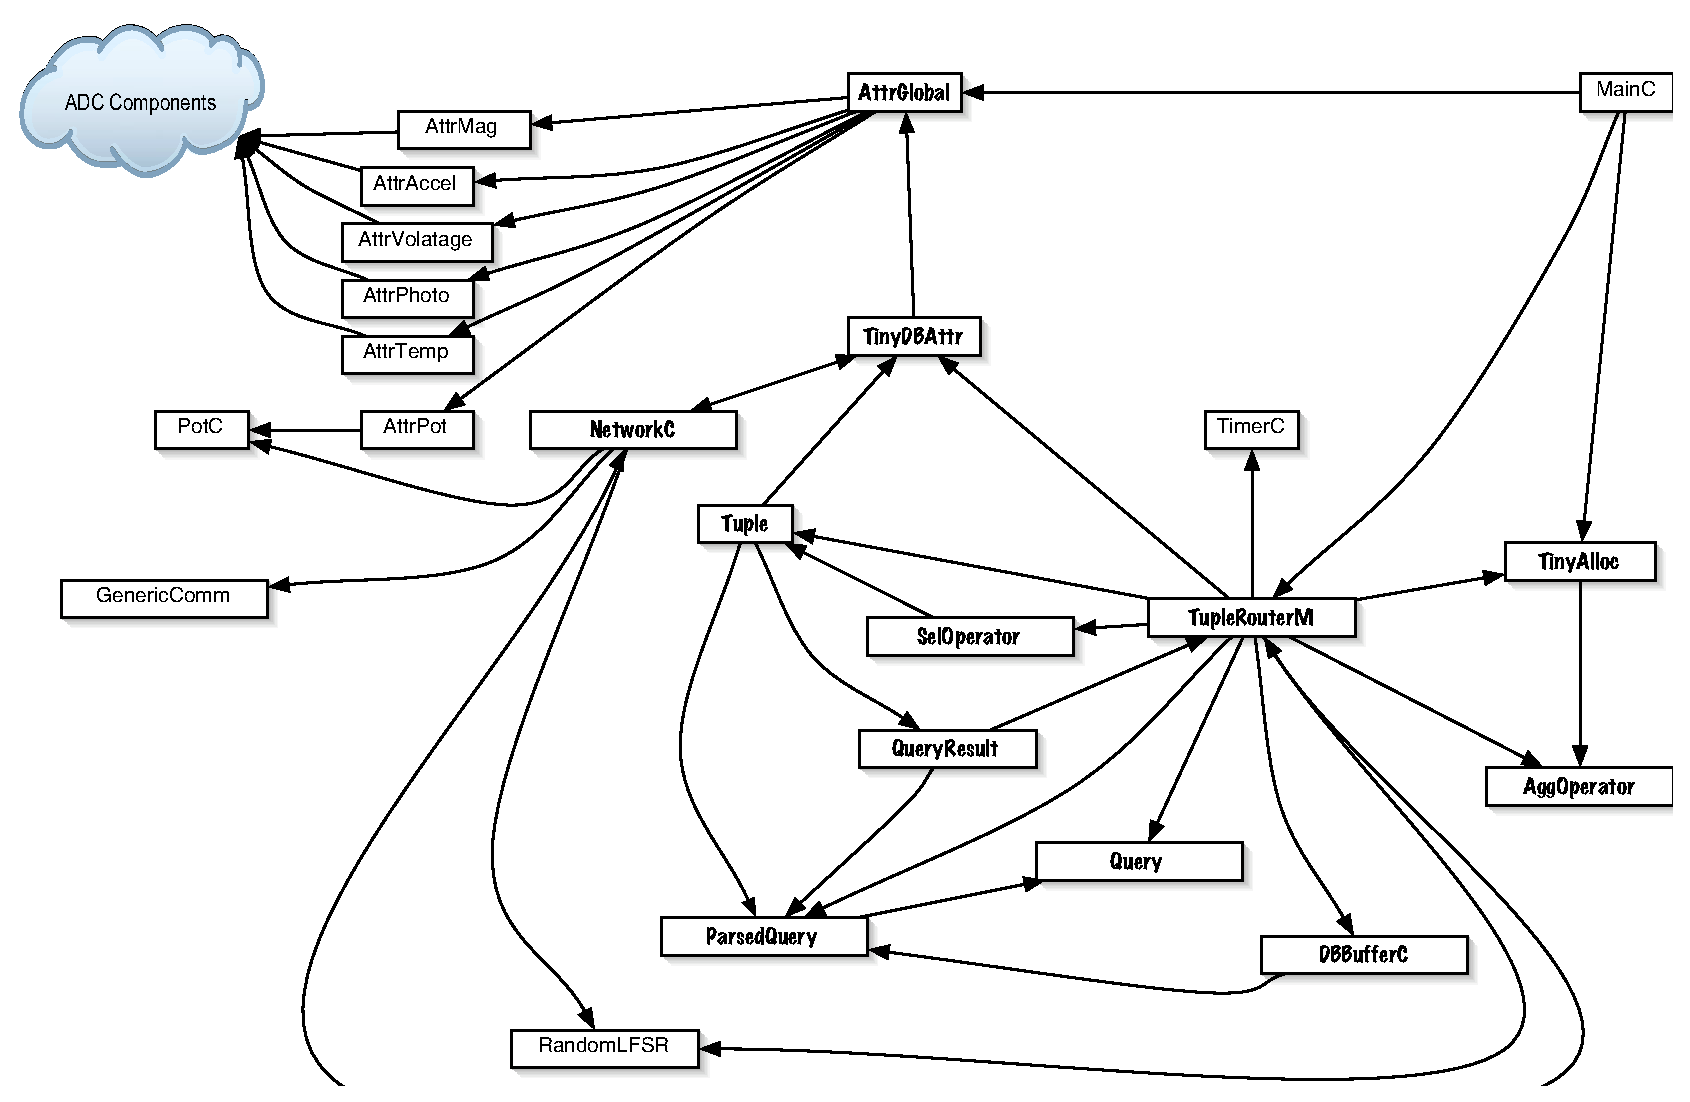
\includegraphics[width=6in]{circuit}
\caption{Component\index{component} diagram.  TinyDB\index{TinyDB}-specific components\index{component} are in the
  bold font.}
\label{fig:components}
\end{figure}

\subsection {The TinyDB\index{TinyDB} Sensor\index{sensor} Catalog\index{catalog} and Schema\index{schema} Manager}
\label{sec:catalog}

A {\em schema\index{schema}} describes the capabilities of the motes\index{mote} in the system as a
single virtual, database ``table\index{table}''.  This table\index{table} can contain any number
of typed {\em attributes\index{attribute}}.  It can also contain handles to a set of
{\em commands} that can be run within the query executor, much like ``methods'' in the Object-Relational\index{Object-Relational}
extensions to SQL\index{SQL}.

During query processing, sensor\index{sensor} readings from each mote\index{mote} are placed
into {\em tuples\index{tuple}}, which may be passed between motes\index{mote} for multi-hop\index{hop}\index{multi-hop}
routing\index{routing} and/or aggregation\index{aggregation}, or which may be passed out the serial port\index{serial}
at the top of the network to the front-end\index{front-end} code.

\subsubsection{\tt Attr and Command\index{schema}\index{Command}\index{Attr}}
\label{sec:schema}
The {\tt Attr\index{Attr}} and {\tt Command\index{Command}} components\index{component} contain the code 
to manage the schema \index{schema} of the mote\index{mote}. The schema consists
of tables\index{table} of
typed attributes\index{attribute} and commands, and associated routines to
update and query these tables.

The {\tt Attr.nc} component implements the {\tt AttrRegister.nc} and {\tt AttrUse.nc} interfaces
for getting and setting the values of attributes.  

Schema\index{schema} commands\index{command} can be invoked locally via ({\tt
CommandUse.invoke}), and to send a message to invoke schema\index{schema}
commands on other nodes\index{node} ({\tt CommandUse.invokeMsg}), both of
which are implemented by the {\tt Command.nc} module.

See the {\em TinySchema} document for complete details on how to manage
attributes and commands for TinyDB.

\subsubsection {\tt TinyDBAttr}
\label{sec:attr}
This simple component\index{component} is the hub for all the
builtin attributes of TinyDB.  It wires all the components that
implement the builtin attributes together.  This component
must be updated if you add a new component that implements
new attributes for TinyDB.

\subsubsection {\tt TinyDBCommand}
\label{sec:command}
This simple component\index{component} is the hub for all the
builtin commands of TinyDB.  It wires all the components that
implement the builtin commands together.  This component
must be updated if you add a new component that implements
new commands for TinyDB.

% {\bf TIP ON EXTENSIONS:}
% If additional attribute\index{attribute} components\index{component} are added to the system, they
% should be added to the initialization code here to make it into the
% schema\index{schema}.

\subsubsection{\tt Tuple\index{tuple}}
This component\index{component} provides fairly straightforward utilities to manage the
{\tt Tuple\index{tuple}} data structure, as defined in {\tt TinyDB.h}.

\subsubsection {\tt QueryResult}
This component\index{component} converts between {\tt Tuple}s\index{tuple}, {\tt QueryResult}s,
and byte-strings.  These data structures are all defined in {\tt
\docroot/tos/lib/TinyDB/TinyDB\index{TinyDB}.h}.  Briefly, a {\tt Tuple}\index{tuple} is a typed vector
of values, as in SQL\index{SQL}; a {\tt QueryResult} holds a tuple\index{tuple} and some
metadata, including the query ID\index{ID}, an index into the result set, and an
epoch\index{epoch} number.

%\subsubsection {\tt MAGNET}
%This component\index{component} is basically a temporary hack to access readings from
%the magnetometers on the Rene motes\index{mote}.  In general, device-specific code
%is to be provided by the general-purpose TinyOS\index{TinyOS} libraries.
%(Section~\ref{sec:devices}).


\subsection{TinyDB\index{TinyDB} Query Processing Operators}
\label{sec:qp}
% \subsubsection {\tt TUPLE\_READER}
\subsubsection {\tt TupleRouter}
This deceptively-named component\index{component} provides the main query processing
functionality on a mote\index{mote}.  As Figure~\ref{fig:components} makes clear,
{\tt TupleRouter} is at the heart of the TinyDB\index{TinyDB} system.  It is called
a tuple\index{tuple} ``router'' because it routes tuples\index{tuple} through a variety of {\em
local} query processing components\index{component}.
% in the spirit of {\em eddies}~\cite{eddies}.  
{\em This component\index{component} does not do network
routing\index{routing}!}  For information on network routing\index{routing} in TinyDB\index{TinyDB}, see 
 Section~\ref{sec:tinydbnetwork}.

The {\tt TupleRouter} component\index{component} contains three main execution
paths:
\begin{itemize}
\item Handling of new query messages
\item Result computation and propagation (each time a clock event goes off)
\item Subtree result message handling
\end{itemize}
We discuss these in turn.

\vspace{1em}
\noindent{\bf Handling New Queries}\\
New queries arrive in {\tt TupleRouter} via the {\tt Network.queryMsg} event.  Each query
  is assumed to be identified by a globally unique ID\index{ID}, which must be
  generated by the Java\index{Java} front-end\index{front-end} APIs\index{API}.  Query
  messages contain a part of a query: either a single field (attribute\index{attribute}) to
  retrieve, a single selection\index{selection} predicate\index{predicate} to apply, or a single
  aggregation\index{aggregation} function to apply.  All the {\tt QueryMessage}s describing a
  single query must arrive before the router will begin routing tuples\index{tuple}
  for that query.

Once all the {\tt QueryMessage}s have arrived, the router calls
  {\tt parseQuery()} to generate a compact representation of the query in
  which field names have been replaced with field IDs\index{ID} that can be used
  as offsets into the sensors\index{sensor} local catalog\index{catalog} ({\tt Schema}\index{schema}).
  
Given a {\tt parsedQuery}, the tuple router allocates space at the end
  of the query to hold a single, ``in-flight'' tuple\index{tuple} for that query --
  this tuple\index{tuple} will be filled in with the appropriate data fields as the
  query executes.
  
{\tt TupleRouter} then calls {\tt setSampleRate()}\index{sample} to start (or restart) the
  mote\index{mote}'s 32khz clock to fire at the appropriate data-delivery rate for
  all of the queries currently in the system.  If there is only one
  query, it will fire once per ``epoch\index{epoch}'' -- if there are multiple queries,
  it will fire at the greatest common divisor of the delivery intervals of all the queries.

\vspace{1em}
\noindent{\bf Tuple\index{tuple} Delivery}\\
Whenever a clock event occurs in {\tt TupleRouter} ({\tt Timer.fired}), the
  router must perform four actions:
\begin{enumerate}

\item Deliver tuples\index{tuple} that were completed on the previous clock event
  ({\tt deliverTuplesTask}).  If the query contains an aggregate\index{aggregate},
  deliver the aggregate\index{aggregate} data from the aggregate\index{aggregate} operator;  if not,
  deliver the tuple\index{tuple} that was filled out during the last
  iteration. Reset the counters that  indicate when these queries
  should be fired again.
  
\item Decrement the counters for all queries.  Any queries whose
  counters reach 0 need to have data delivered.  Reset the
  expression\index{expression}-specific state for these queries (this is specific
  to the expressions\index{expression} in the queries -- {\tt MAX} aggregates\index{aggregate}, for instance,
  will want to reset the current maximum aggregate\index{aggregate} to some large
  negative number.)

\item Fetch data fields for each query firing this epoch\index{epoch}.  Loop
  through all fields of all queries, fetch them (using the {\tt Schema\index{schema}}
  interface), and fill in the appropriate values in the tuples\index{tuple}
  on the appropriate queries.  
  
\item Route\index{routing} filled-in tuples\index{tuple} to query operators.  First route to
  selections\index{selection}, then the aggregate\index{aggregate} (if it exists).  If any selection\index{selection}
  rejects a tuple\index{tuple}, discard it.

\end{enumerate}

\vspace{1em}
\noindent{\bf Neighbor\index{neighbor} Result Arrival}\\
  When a result arrives from a neighbor\index{neighbor}, the {\tt TupleRouter} receives a {\tt Network.dataMsg} event.
  This result needs to be integrated into the aggregate\index{aggregate} values being computed
  locally.  If the result corresponds to an aggregate\index{aggregate} query, that result
  is forwarded into the {\tt AggOperator} component\index{component}, otherwise it is 
  simply forwarded up the routing\index{routing} tree towards the root\index{root}.

\subsubsection {\tt SelOperator}
The {\tt SelOperator} is responsible for relational\index{relational} {\em
selection\index{selection}}: testing whether tuples\index{tuple} match predicates\index{predicate} (in task {\tt
doFilter\index{filter}}). Currently, the only expressions\index{expression} supported are standard
arithmetic\index{arithmetic} comparisons of attributes\index{attribute} with constants.

\subsubsection {\tt AggOperator}
This component\index{component} performs two SQL\index{SQL} features: {\tt GROUP BY}\index{Group By}\index{group} and
aggregation\index{aggregation}.

The optional {\tt GROUP BY}\index{Group By}\index{group} feature partitions the data by the value
of a (set of) attribute\index{attribute}(s).  Aggregate\index{aggregate} functions are computed for each
partition, over any attributes\index{attribute} {\em not} in the {\tt GROUP BY}\index{Group By} clause.  In
the absence of a {\tt GROUP BY}\index{Group By} expression\index{expression}, the aggregate\index{aggregate} is computed
over all tuples\index{tuple}.  As described in Section~\ref{sec:queries}, aggregate\index{aggregate}
results are updated once per ``epoch\index{epoch}''.

The code in this component\index{component} needs to (a) take readings from the current
node\index{node} ({\tt Operator.processTuple}), (b) merge those readings
with sub-aggregates\index{aggregate} from the subtree ({\tt
Operator.processPartialResult}), and (c) return this node's\index{node}
sub-aggregate\index{aggregate} results up the tree ({\tt Operator.nextResult}).
It also manages allocating aggregation\index{aggregation} state for each group\index{group} using the
{\tt TinyAlloc} component\index{component} (Section~\ref{sec:tinyalloc}), and
provides a utility to reset the running aggregation\index{aggregation} state ({\tt
Operator.resetExprState}).

\subsection {{\tt TinyAlloc}: The TinyDB\index{TinyDB} Memory Manager}
\label{sec:tinyalloc}
This component\index{component}, being very general-purpose, is located in {\tt
\docroot/tos/shared/TinyAlloc.\{c,comp\}} for use by other applications.

TinyAlloc is a simple, handle-based\index{handle} compacting memory manager.  It
allocates bytes from a fixed size frame and returns handles (pointers
to pointers) into that frame.  Because it uses handles, TinyAlloc can
move memory around in the frame without changing all the external
references.  Moving memory is a good thing because it allows frame
compacting and tends to reduce wasted space.  Handles can be accessed
via a double dereference (**), and a single dereference can be used
wherever a pointer is needed, but if a single dereference is to be
stored, the handle must be locked first (via {\tt MemAlloc.lock(h)}),
as otherwise TinyAlloc may move the handle and make the reference
invalid.  

\vspace{.1in}
\renewcommand{\baselinestretch}{1.0}\rm
\fbox{\parbox{.9\columnwidth}{
{\bf BEWARE:} Passing around dereferenced handles without locking
is a common source of bugs, as are problems that result from
memory not being unlocked.
}}
\renewcommand{\baselinestretch}{1.2}\rm
\vspace{.1in}

   Like all good TinyOS\index{TinyOS} programs, TinyAlloc is
   split-phase\index{split phase} with
respect to allocation and compaction.  Allocation/reallocation
completion is signalled via a {\tt MemAlloc.allocComplete()} signal and
compaction via a {\tt MemAlloc.compactComplete()} signal.  All other
operations complete and return in a single phase. Note that compaction
may be triggered automatically from allocation; in this case a
{\tt compactComplete}  event is not generated.

Handles\index{handle} are laid out in the frame as follows:
\begin{verbatim}
   [LOCKED][SIZE][user data] 

Where: 
    LOCKED     : a single bit indicating if the handle is locked 
    SIZE       : 7 bits representing the size of the handle 
    user data  : user-requested number of bytes (**h) points to
                 [user data], not [LOCKED].
\end{verbatim}
   Calling {\tt MemAlloc.size(h)} returns the size of {\tt [user
data]} (note that the internal function {\tt size()} returns the size of the
entire handle, including the header byte.)

\subsection{TinyDB\index{TinyDB} Multihop Routing\index{routing}} \label{sec:tinydbnetwork}

TinyDB includes a modular interface for interacting with a number of different
multihop routing layers.  This interface, called {\tt Network.nc} is 
available in {\tt \docroot/tos/lib/TinyDB/}, requires routing layers
to provide the following methods:
\begin{itemize}
\item {\tt command QueryResultPtr getDataPayLoad(TOS\_MsgPtr msg)}:  Command used to get the start of
a query result from a message pointer.  This can be used to write a query result into a message,
or extract results from a message received over the radio.  TinyDB guarantees it will call this before
reading or writing query results from any data message, so that the routing layer can ensure that
sufficient space appears at the beginning of the message for its internal headers.
\item {\tt command TinyDBError sendDataMessage(TOS\_MsgPtr msg)}:  Command used to send a data message.
Data messages are transmitted to the root of the network, which is defined by the routing layer.
TinyDB requires that the routing layer be duplicate-free, but it is otherwise free to use any
routing mechanism it desires.
\item {\tt command QueryMessagePtr getQueryPayLoad(TOS\_MsgPtr msg)}: Similar to {\tt getDataPayload},
returns the offset in a message buffer that should be used for reading or writing a query message.
\item {\tt command TinyDBError sendQueryMessage(TOS\_MsgPtr msg)}:  Command used to flood a query
message throughout the network.  TinyDB expects that this will be sent via a local broadcast -- 
the application takes care of rebroadcasting the message to ensure that all nodes in the network
receive it.
\item {\tt event result\_t sendQueryDone(TOS\_MsgPtr msg, result\_t success)}:  Event that is signaled
when a {\tt sendQueryMessage} command completes.
\item {\tt event result\_t sendDataDone(TOS\_MsgPtr msg, result\_t success)}:  Event that is signaled
when a {\tt sendDataMessage} command completes.
\item {\tt event result\_t dataSub(QueryResultPtr qresMsg)}:  Event that is signaled when a data message
arrives from another sensor; not that this message must have been directed locally to the node.
\item {\tt event result\_t querySub(QueryMessagePtr qMsg)}:  Event that is signaled when a query 
message is received from another sensor.
\item {\tt event result\_t snoopedSub(QueryResultPtr qresMsg, bool isFromParent, uint16\_t senderid)}:
Event that is signaled when a non-locally addressed data message is overheard over the radio.  
\end{itemize}
The default multihop routing layer in TinyDB is implemented by the 
{\tt \docroot/tos/lib/TinyDB/NetworkMultiHopM.nc} components, which provides
a wrapper on the standard TinyOS multihop routing component in {\tt /docroot/tos/lib/Route}.

%% The {\tt Network} component\index{component} handles all the
%% mote-to-mote\index{mote} and mote-to-serial-port\index{serial}
%% communication for TinyDB\index{TinyDB}, routing\index{routing} {\em
%%   query} and {\em data} messages.  In doing so, it also participates
%% in a distributed algorithm for network topology\index{topology}
%% layout.  Messages are all of type {\tt TOS\_Msg}, and begin with a
%% {\tt DBMsgHdr} structure (see {\tt
%%   \docroot/tos/include/TinyDB\index{TinyDB}.h}), followed by a
%% payload.

%% \vspace{1em}
%% \noindent {\bf Topology\index{topology} Maintenance}\\ Most of the code in this
%% component\index{component} manages the network
%% topology\index{topology}.  The network topology\index{topology} is
%% maintained as a routing\index{routing} {\em tree}, with
%% Mote\index{mote} \#0 at the root\index{root}.  As a rule, query
%% messages flood down the tree in a straightforward fashion.  Data
%% messages flow back up the tree, participating in more complex query
%% processing algorithms.  Mote\index{mote} \#0 passes result data to the
%% front-end\index{front-end} code via its serial\index{serial}
%% interface.  The only exception to ``query-down/data-up'' rule is that
%% the root\index{root} itself sends out periodic (empty) data messages
%% as a ``heartbeat''\index{heartbeat}, so that its communication
%% abilities can continue to be measured while a query runs.

%% By default, a simple tree-maintenance algorithm is used.  This
%% algorithm has each mote\index{mote} keep track of a list of other
%% motes\index{mote} from which it receives messages ({\em
%%   neighbors\index{neighbor}}).  Among these neighbors\index{neighbor},
%% it chooses the best one as its {\em parent\index{parent}} in the tree.
%% Alternatively (for testing purposes) the network can be forced to
%% choose a static topology\index{topology} based on the numbering of the
%% nodes\index{node}.  This is done via the {\tt forceTopology()}
%% command.

%% \vspace{1em}
%% \noindent{\bf Message Handling}\\
%% Upon receiving a message on the network, this
%% component\index{component} invokes the internal routine {\tt
%%   processHeader}, which examines the header of each packet received on
%% the radio.  This code drives much of the logic in the
%% component\index{component}.  It first updates statistics that are
%% maintained for the parent-choice logic, and updates its choice of
%% parent\index{parent} if necessary.  Then, if the message is a data
%% message destined for another node\index{node}, it drops the message.
%% Otherwise, it handles the message accordingly.

\subsection{TinyOS\index{TinyOS} Service Components\index{component}}
We describe these TinyOS\index{TinyOS} services only briefly.  For
more detail see TinyOS\index{TinyOS}.
\begin{itemize}
\item {\tt Clock}: Provides a system clock, and clock interrupts.
\item {\tt GenericComm}: A generic communications layer, supporting
  radio and serial\index{serial} communication.
\item {\tt Leds}: Control of the LED indicators on the motes\index{mote}.
\item {\tt Main}: A shell to initialize subordinate modules, and start
  them up.
\item {\tt Pot}: Get and set the level of the potentiometer
  (transmission-power controller) on the radio.
\item {\tt RandomLFSR}: A psuedo-random number generator, based on a
  16-bit Linear Feedback Shift Register.
\item {\tt Reset}:  Reset a mote\index{mote} (equivalent to toggling the 
power switch.)
\item {\tt Timer}: A service for setting (multiple) timers to generate
  subsequent interrupts.
\end{itemize}

%\subsection{Attributes\index{attribute}: Sensor\index{sensor} Components\index{component} and Introspection\index{introspection}}
%\label{sec:devices}
%We describe these TinyOS\index{TinyOS} services only briefly.  For
%more detail see TinyOS\index{TinyOS}.
%\begin{itemize}
%\item {\tt Accel}: Accelerometer: measures movement in two dimensions
%  (X and Y).
%\item {\tt Mag}: Magnetometer: measures magnetic field.
%\item {\tt Photo}: Light sensor\index{sensor}.
%\item {\tt Temp}: Thermometer: measures temperature.
%\item {\tt Voltage}: Measures remaining voltage in the
%  battery\index{battery}.
%\end{itemize}
%\section{Background}
%\subsection{Related Reading}
%\subsection{In-Network Processing\index{in-network}}
%\subsection{Declarative Query Processing}


\section{Running TinyDB in the TOSSIM Simulator}\label{sec:tossim}\index{TOSSIM}

TinyDB includes support for the TinyOS simulator, TOSSIM (also know as
``nido'').  Running under TOSSIM requires recompilation of the java
source code as well as the mote code, and requires passing a special
flag to the TinyDB java application when it is started.  See the file
{\tt \docroot/doc/nido.pdf} for more information about TOSSIM.  The
basic steps to set up TinyDB for TOSSIM are as follows:

\begin{itemize}
\item Recompile the java code by typing {\tt make clean; make -f
    MakePC} in the {\tt \docroot/tools/java/net/tinyos/tinydb}
  directory.  This will rebuild all of the TinyDB source code,
  ensuring that the messaging classes are configured to talk with the
  simulator.
\item Compile the PC binary from the {\tt TinyDBApp} application by
  typing {\tt make -f MakePC pc} in the {\tt \docroot/apps/TinyDBApp}
  directory.
\item Set the DBG string variable appropriately; for example {\tt
    export DBG=usr1}.
\item Start the PC binary with $n$ simulated motes by typing {\tt
    ./build/pc/main.exe n} in the {\tt \docroot/apps/TinyDBApp}
  directory.
\item Start the java GUI in simulator mode by typing (in a different
  shell window) {\tt java net.tinyos.tinydb.TinyDBMain -sim} in the
  {\tt \docroot/tools/java} directory.
\item Assuming you set the DBG string as above, you should be able to
  click the ``Reset Motes'' button a see a message in the window where
  you started the PC binary stating that reset is not support in the
  simulator.
\end{itemize}

\subsection{Adding a New Aggregate Operator}\label{sec:adding-aggs}\index{Aggregates, Adding}

TinyDB includes a facility to make it relatively easy for programmers
to author new aggregate operators.  See the accompanying manual,
``Extending TinyDB: Creating Custom Aggregates'' included with the
TinyOS-1.1 release and available on the TinyDB web page for more
information.

\section{Using the TinyDB GUI with PostgreSQL}\label{postgres}\index{PostgreSQL}

Though TinyDB still supports these logging features, it is highly
recommended that users interested in long-term deployments based on
TinyDB use the TASK\index{TASK, Application Sensor Kit} client
(documentation for TASK is available from the TinyDB website.) TASK
supports much more thorough logging and configuration management than
the features described below.

TinyDB includes a simple facility to log results of queries to a
PostgreSQL\index{PostgresQL} database.  Postgres is an open-source,
widely used DBMS available on a wide-variety of platforms ( See
\htmladdnormallink{{\tt
www.us.postgresql.org}}{http://www.us.postgresql.org} for more
information.)  To enable logging to a Postgres database, set up
Postgres according to the directions in the next section, and then
enable the ``Log to Database'' option when inputting a query via the
query GUI (see Figure \ref{fig:query}.) Note that it is not neccessary
to configure Postgres {\it unless you wish to use the logging
facilities}.  The results of the query will be written to a table
named ``q$n$'', where $n$ is a unique sequence number assigned to the
query.  You can determine the current sequence number for a query by
calling the {\tt getTableName()} method on the {\tt DBLogger} object
used to initiate query logging.  The resulting table will contain a
timestamped entry for each result returned by the query.  For example,
if your query is {\it select light,temp from sensors}, the resulting
Postgres table will have the schema:

\begin{tabular}{|c|c|c|c|}
\hline
{\tt result\_time:timestamp} & {\tt epoch:integer}&{\tt light:integer}&{\tt temp:integer} \\
\hline
\end{tabular}

\noindent In this way, TinyDB query results can be accessed offline and joined with results from other static, offline data sources.

\subsection{Configuring PostgreSQL}\label{sec:postgres-config}\index{PostgreSQL, Configuring}
The following is a simple guide for installing and configuring
Postgres \index{Postgres} to support logging of TinyDB queries.  We
have successfully used TinyDB with Redhat Linux 7.2 and 7.3 and
Cygwin; other Linux distributions should be straightforward to
configure.  Section \ref{sec:redhat} provides installation
instructions for Linux;  Section \ref{sec:cygwin} gives
instructions for Cygwin under Windows.


\subsubsection{Redhat Linux}\label{sec:redhat}\index{linux}\index{Redhat}

\begin{enumerate}
\item{\bf Download and Install PostgreSQL}

Download Postgres for your distribution from \\
\htmladdnormallink{ftp://ftp3.us.postgresql.org/pub/postgresql/binary/v7.3.4/RPMS/}{ftp://ftp3.us.postgresql.org/pub/postgresql/binary/v7.3.4/RPMS/}.  
You'll need at least the following packages:

{\tt
postgresql-libs \\
postgresql \\
postgresql-server \\
postgresql-jdbc \\
}

Note that newer versions of Redhat linux come with the {\tt
postgresql} and {\tt postgres-libs} packages preinstalled, but with
versions older than 7.3.4.  You will either need to remove these
packages before installing the 7.3.4 packages, or just install the
{\tt postgresql-server} and {\tt postgres-jdbc} packages from the
version of Postgres that came with your Redhat distribution.

Install the packages in the above order, and then start the Postgres
service.  Under Redhat, the command to do this is: {\tt
/etc/rc.d/init.d/postgresql start}

\item{\bf Enable Remote Connections}

You'll need to modify your Postgres installation to allow connections over TCP/IP sockets.  With the Redhat RPMS, Postgres
is configured to store its data files in {\tt /var/lib/pgsql/data};  you'll need to substitute appropriately in the
commands below if your Postgres files are in a different location:

\begin{itemize}

\item {\tt cd /var/lib/pgsql/data}
\item Edit {\tt postgresql.conf} by
replacing the line (at the end of the comments section) that reads: \\
{\tt \#tcpip\_socket = false} \\
with \\
{\tt tcpip\_socket = true} \\
\item Restart the postgresql server (under Redhat, type {\tt /etc/rc.d/init.d/postgresql restart})
\end{itemize}

On some Redhat installations, you may also need to enable connections from localhost (e.g. IP address 127.0.0.1).  To do this:

\begin{itemize}
\item Edit {\tt pg\_hba.conf} by
adding the following line to the end of the file: \\

{\tt \#tcpip\_socket = false} \\
with \\
{\tt tcpip\_socket = true} \\
\item Restart the postgresql server (under Redhat, type {\tt /etc/rc.d/init.d/postgresql restart})
\end{itemize}



\item{\bf Install the PostgreSQL JDBC driver}

Next, you'll need to make sure the Postgres JDBC driver (included in the TinyOS distribution) is in your classpath.  The
jar is located at \java/jars/pgjdbc2.jar;  under bash, you would type:

{\tt export CLASSPATH=\$CLASSPATH:\java/jars/pgjdbc2.jar}

\item{\bf Create the TinyDB User and Database}

The TinyDB config file (see \ref{sec:configfile}) above specifies a database and user name to use when accessing 
Postgres.  Both need to be created before TinyDB will work;  to do this under Redhat, type:

{\tt
su \\
postgres \\
createdb tinydb \\
createuser tele \\
}

\item{\bf Create the Queries Table}

TinyDB logs all of the queries that are logged to a table ``queries'', which contains the name of the result table
for the query,  time
the query was posed, and the text of the query.  You must create this table before TinyDB;
to do so under Redhat, do the following:

\begin{itemize}
\item {\tt su; su postgres}
\item Get a Postgres command prompt by typing: {\tt psql tinydb}
\item Create the table by typing: {\tt create table queries (query\_table varchar(10), query\_time timestamp, query\_string varchar(500));}
\end{itemize}
\end{enumerate}

\subsubsection{Cygwin}\label{sec:cygwin}\index{Cygwin}

\begin{enumerate}
\item{\bf Initialize PostgreSQL} 
{\it Note:  This step is only neccessary if you have never used Postgres under Cygwin.}

You need to choose a directory where Postgres will store its data files.  We'll
use {\tt /pgdata}, though you may choose any directory.

Before running Postgres, you must install the cygipc \index{cygipc}  package (note that this may change
for future releases of Cygwin.)  We have verified that cygipc 1.14 works.

Cygipc is now part of the cygwin distribution available from \htmladdnormallink{http://www.cygwin.com}{http://www.cygwin.com}. 

Initialize Postgres using the following commands:

\begin{itemize}
\item {\tt export PGDATA=/pgdata}
\item {\tt mkdir /pgdata}
\item {initdb}
\end{itemize}

This may take several seconds to complete.  You should see several lines of output
about creating directories and fixing permissions.

You may wish to modify your Windows environment to set these variables and start the
ipc-daemon automatically.  You can add the ``{\tt export PGDATA=/pgdata}'' command to
your .bashrc file.  To cause the ipc-daemon to be started whenever windows boots,
run the command ``{\tt ipc-daemon --install-as-service}''.

To use Postgres, you need to start the postmaster daemon -- type {\tt pg\_ctl start}
to start it. Note that you must do this every time you wish to use Postgres
features after having restarted your machine.

\item{\bf Enable Remote Connections}

You'll need to modify your Postgres installation to allow connections
over TCP/IP sockets:

\begin{itemize}

\item {\tt cd \$PGDATA/}
\item Edit {\tt postgresql.conf} by
replacing the line (at the end of the comments section) that reads: \\
{\tt \#tcpip\_socket = false} \\
with \\
{\tt tcpip\_socket = true} \\
\item Restart the postgresql server by typing {\tt pg\_ctl restart})
\end{itemize}

\item{\bf Install the PostgreSQL JDBC driver}

Next, you'll need to make sure the Postgres JDBC driver (included in the TinyOS distribution) is in your classpath.  The
jar is located at \java/jars/pgjdbc2.jar;  under bash, you would type:

{\tt export CLASSPATH=\$CLASSPATH:\java/jars/pgjdbc2.jar}

\item{\bf Create the TinyDB User and Database}

The TinyDB config file (see \ref{sec:configfile}) above specifies a database and user name to use when accessing 
Postgres.  Both need to be created before TinyDB will work;  to do this under, type:

{\tt
createdb tinydb \\
createuser tele \\
}

\item{\bf Create the Queries Table}\index{Queries Table}

TinyDB logs all of the queries that are logged to a table ``queries'', which contains the name of the result table
for the query,  time
the query was posed, and the text of the query.  You must create this table before TinyDB;
to do so, do the following:

\begin{itemize}
\item Get a Postgres command prompt by typing: {\tt psql tinydb}
\item Create the table by typing: {\tt create table queries (query\_table varchar(10), query\_time timestamp, query\_string varchar(500));}
\end{itemize}
\end{enumerate}


\section{Frequently Asked Questions}

\begin{itemize}
\item{\bf I'm using a Serial Forwarder and TinyDBMain complains that it can't connect to the network
        when I try to start it.  Why doesn't it find my Serial Forwarder?}

TinyDB is configured to connect directly to the network.  You can make it use an
existing serial forwarder by changing the value of the {\tt comm-string} in the tinydb.conf
file (see Section \ref{sec:configfile}) to {\tt sf@localhost\$9000}.  You'll need to change
the port number and host name appropriately.

\item{\bf I've installed TinyDB on my motes and connected them to the basestation, but I can't ever seem
        to get them to send or process queries.  What's going on?}

First (as always), check that all your cables are properly connected.  Power cycle your base station.
If you still can't send queries, verify that the {\tt comm-string}  
field in the tinydb.conf file (see Section \ref{sec:configfile}) 
is set correctly according to {\tt \docroot/doc/serialcomm/index.html}.
A common problem is the wrong setting of the UART baud rate.
The correct baud rates are 19200 for mica and mica2dot,
57600 for mica2.

%\item{\bf I send a query into the network.  I get results back for a short period of time, but then
%stop receiving any results.  The motes are all blinking their red and green LEDS like crazy. 
%What's going on?}
%
%You're probably running a query with a fast epoch duration.  The basestation periodically broadcasts
%heartbeats that tell the motes it's still alive, but the motes can lose track of the basestation
%if they are sending data very fast.  You can work around this problem by using the ``Change Base Bcast 
%Interval'' button on the TinyDB command window just after injecting the query.

\item{\bf I think I've found a bug in TinyDB. What should I do?}
There is a bug tracker for TinyDB in the TinyOS sourceforge project, under ``Trackers''.
Check out the URL:

\htmladdnormallink{http://sourceforge.net/tracker/?atid=494883\&group\_id=28656\&func=browse}{http://sourceforge.net/tracker/?atid=494883\&group\_id=28656\&func=browse} 

for a list of bugs that have
been submitted.  If you see a similar bug there, we may have posted a workaround.  If your bug isn't
there, or the workaround is not satisfactory, feel free to enter a new bug or send us a bug report and
we'll enter it for you!

\end{itemize}
\section{Version History and Author Information}


This document was written by Joe Hellerstein, Sam Madden, and Wei Hong.  This
is Version 0.4, last updated September 17, 2003.


{\it Changes in version .4}: Updated documentation for the TinyOS 1.1 release.

{\it Changes in version .31}:   Updated documentation on using Postgres with Windows/Cygwin.


%\section{The TinyDB\index{TinyDB} License}

\appendix

\section{TinyDB Source Files}
\label{app:files}
The following files in the TinyOS CVS tree are a
part of the TinyDB\index{TinyDB} distribution:

\renewcommand{\baselinestretch}{.9}\rm
\begin{itemize}
\item {\tt \docroot/tos/lib/TinyDB}
\begin{itemize}
\item {\tt /AggOperator.rd}
\item {\tt /DBBufferC.nc}
\item {\tt /DBBuffer.nc}
\item {\tt /DBBuffer.h}
\item {\tt /ExprEvalC.nc}
\item {\tt /ExprEval.nc}
\item {\tt /NetworkC.nc}
\item {\tt /Network.nc}
\item {\tt /Operator.nc}
\item {\tt /ParsedQueryIntf.nc}
\item {\tt /ParsedQuery.nc}
\item {\tt /QueryIntf.nc}
\item {\tt /Query.nc}
\item {\tt /RadioQueue.nc}
\item {\tt /SelOperator.nc}
\item {\tt /TinyDBAttr.nc}
\item {\tt /TinyDBCommand.nc}
\item {\tt /TinyDB.h}
\item {\tt /TupleIntf.nc}
\item {\tt /TupleRouter.nc}
\item {\tt /TupleRouterM.nc}
\item {\tt /Tuple.nc}
\end{itemize}
\item {\tt \docroot/tos/interfaces}
\begin{itemize}
\item {\tt /Attr.h}
\item {\tt /AttrRegisterConst.nc}
\item {\tt /AttrRegister.nc}
\item {\tt /AttrUse.nc}
\item {\tt /Command.h}
\item {\tt /CommandRegister.nc}
\item {\tt /CommnadUse.nc}
\item {\tt /MemAlloc.nc}
\item {\tt /SchemaType.h}
\end{itemize}
\item {\tt \docroot/tos/lib}
\begin{itemize}
\item {\tt /Command.nc}
\item {\tt /Attr.nc}
\item {\tt /TinyAlloc.nc}
\end{itemize}
\item {\tt {\java}/net/tinyos/tinydb}
\begin{itemize}
\item {\tt AggExpr.java}
\item {\tt AggOp.java}
\item {\tt Catalog.java}
\item {\tt CmdFrame.java}
\item {\tt CommandMsgs.java}
\item {\tt MagnetFrame.java}
\item {\tt QueryExpr.java}
\item {\tt QueryField.java}
\item {\tt QueryListener.java}
\item {\tt QueryResult.java}
\item {\tt ResultFrame.java}
\item {\tt ResultGraph.java}
\item {\tt ResultListener.java}
\item {\tt SelExpr.java}
\item {\tt SelOp.java}
\item {\tt TinyDBCmd.java}
\item {\tt TinyDBMain.java}
\item {\tt TinyDBNetwork.java}
\item {\tt TinyDBQuery.java}
\item {\tt Makefile}
\item {\tt parser/}
\begin{itemize}
\item {\tt Makefile}
\item {\tt senseParser.\{cup,lex\}}
\end{itemize}
\end{itemize}
\item {\tt {\docroot}/apps/TinyDBApp}
\begin{itemize}
\item {\tt Makefile}
\item {\tt TinyDBApp.nc}
\end{itemize}
\end{itemize}
\renewcommand{\baselinestretch}{1.2}\rm

\begin{latexonly}
% Glossary entries
\nomenclature{\bf Active Messages (AM)}{A networking protocol developed at
  UC Berkeley, used for very-low-latency dispatch of incoming
  messages.  It provides an asynchronous (sometimes called
  ``split-phase'') programming model.\\}
\nomenclature{\bf Aggregation}{Aggregation is the process of
  bringing together multiple data objects.  In SQL, it typically
  denotes the summarization of multiple numeric values with a single
  summary statistic, like COUNT, AVG, MAX or MIN.\\}
\nomenclature{\bf API}{Application Programming Interface.  A set of
  interfaces provided by a subsystem that enable programmers to use
  the subsystem in their own applications.\\ }
\nomenclature{\bf Attribute}{In traditional databases, a row in a table,
  consisting of a name and a data type.  In TinyDB, an attribute often
  corresponds to a physical sensor reading like light, temperature,
  etc.  However, the system can support attributes provided in
  software as well, like NodeID\index{ID}, network parent\index{parent}, and so on.}
\nomenclature{\bf Catalog}{A set of metadata describing a database,
  including the schema, and whatever other metadata the system
  provides.}
\nomenclature{\bf Client}{In the TinyDB context, a piece of code running
  on a PC that invokes the TinyDB Java API.  Synonym for Front-End.}
\nomenclature{\bf Column}{See Attribute.}
\nomenclature{\bf COM1}{The name of the standard serial port on a PC.}
\nomenclature{\bf Component}{A basic building block in a TinyOS
  program. See the TinyOS documentation for details on the TinyOS
  programming model.}
\nomenclature{\bf Declarative Language}{A language in which you
  express what you desire, without detail on how to achieve it.
  Declarative languages are popular in database systems; SQL is
  (largely) declarative.  Declarative languages are useful for providing a
  very deep level of indirection between application requests and
  system implementation of the requests -- this is especially important if the
  system's optimal implementation could change frequently (as in a
  sensor network, which is quite unpredictable).}
\nomenclature{\bf Download}{In the context of TinyOS/TinyDB, this is the
  process of transfering a compiled code image onto a mote.}
\nomenclature{\bf Embedded C}{A program written in C that runs
  autonomously on a small device like a mote.} 
\nomenclature{\bf Epoch}{A discrete window of time.  In TinyDB's SQL, new
  answers to a query are produced every epoch, and the duration of an
  epoch can be specified in the query.}
\nomenclature{\bf Expression}{A simple interpretable clause in a query,
  like an arithmetic comparison (e.g.\ {\tt light $>$ 80}), or an
  aggregate function (e.g.\ {\tt AVG(temp)})}.
\nomenclature{\bf Filter}{A predicate that may remove some readings from
  the query.  Synonym for Selection.}
\nomenclature{\bf Front-End}{In the TinyDB context, a piece of code running
  on a PC that invokes the TinyDB Java API.  Synonym for Client.}
\nomenclature{\bf Group By}{In SQL, an expression that partitions the set of
  tuples that satisfy a query, to prepare for computation of an
  aggregate per partition.  Typically the Group By expression is
  simply an attribute name, e.g.\ {\tt GROUP BY temp}; tuples are
  partitioned by the value of the attribute.}
\nomenclature{\bf GUI}{Graphical User Interface.}
\nomenclature{\bf Handle}{A pointer to a pointer to an object.  The
  double level of indirection allows the objects to be relocated
  without informing the code that manipulates the handles.}
\nomenclature{\bf Heartbeat}{A periodic network message that simply
  indicates that the sender is active and connected.}
\nomenclature{\bf In-Network}{A description for algorithms that run in
  intermediate network devices in a multi-hop network, rather than the
  hosts at the endpoints.}
\nomenclature{\bf Listener}{A Java object that responds to certain
  kinds of events.}
\nomenclature{\bf Mote (Berkeley Mote)}{A wireless sensor network
  node, developed at UC Berkeley.  A mote is a device combining a small
  microprocessor, one or more sensors, and a radio.  The name ``mote''
  comes from the ``Smart Dust'' metaphor introduced by sci-fi author Neal Stephenson.}
\nomenclature{\bf Multi-Hop}{A scenario in which network messages
  visit multiple routers between source and destination.}
\nomenclature{\bf Neighbor}{Two network nodes are neighbors if they
  can communicate directly, without involving any intermediate routing.}
\nomenclature{\bf Node}{In this context, a compute device in a
  network; typically a mote in a sensor network.}
\nomenclature{\bf Object-Relational}{A database model developed in the
  Postgres project at UC Berkeley, which extends the
  relational model with object-oriented features like extensible
  abstract data types, including OO methods that are executed by the
  database engine (rather than at a client).}
\nomenclature{\bf Parent}{In a TinyDB routing tree, the parent of node
  $n$ is the node that listens to $n$'s data messages.}
\nomenclature{\bf Predicate}{A boolean expression.}
\nomenclature{\bf Processed}{In the TinyDB API, a result tuple is considered
  ``processed'' when all the attributes have been concatenated
  together with fully aggregated values.}
\nomenclature{\bf
  Ptolemy}{\htmladdnormallink{Ptolemy}{http://ptolemy.eecs.berkeley.edu}
  is a simulation project at UC Berkeley.  The TinyDB application
  borrows a small piece of code from 
  Ptolemy for plotting results.} 
\nomenclature{\bf Query Plan}{An interpretable description for
  executing a query, typically consisting of a few high-level
  operators connected in a dataflow tree.}
\nomenclature{\bf Query Processor}{A system for executing queries.}
\nomenclature{\bf Relational Model, Relational Languages}{Invented by
  Turing Award-Winner Ted Codd, the
  relational data model is the most prevalent representation for data
  today.  It is extremely simple, representing all information as
  relations (``tables'') consisting of tuples (``rows'') made up of
  well-typed attributes (``columns'').  A relational query language is
  one that can express a subset of 1st-order logic over relations.
  The standard relational query language is SQL.}
\nomenclature{\bf Root}{In TinyDB, this refers to the root of the
  routing tree, which is a sensor that is connected to the serial port
  of the PC running the front-end code.}
\nomenclature{\bf Routing}{The process of moving data through a
  multi-hop network from source to destination.  In TinyDB, the
  dataflow involved in routing interacts significantly with the
  dataflow involved in query processing.}
\nomenclature{\bf Row}{See Tuple.}
\nomenclature{\bf Sample}{In the sensor context, this often refers to
  a single discrete reading taken by a sensor.  It is called a sample to highlight
  the approximate nature of representing a continuous, real-world
  process as a stream of discrete digital readings.}
\nomenclature{\bf Schema}{A metadata description of a relation or set of
  relations.  A simple schema includes the name of the relation(s), the
  names and data types of the attributes in the relation, and the
  default order of the attributes.  Note that the schema describes
  what data {\em can} exist in the relation, not what {\em currently}
  exists.}
\nomenclature{\bf Selection}{In relational languages, the operation of
  choosing those tuples in a relation that match some predicate.  See Filter.}
\nomenclature{\bf Semantics}{The meaning of a construct.}
\nomenclature{\bf Sensor}{A device for converting physical phenomena into
     electronic signals.  In this document we sometimes use the word sensor
     interchangeably with the word mote: the combination of a sensor, a
     processor, and a radio.}  
\nomenclature{\bf Sensor Network}{A network -- often a wireless
  network -- in which the nodes are devices like motes that combine
  sensors with processing and commmunication.}
\nomenclature{\bf Serial Port}{An I/O port present on most PCs.}
\nomenclature{\bf SQL}{The Structured Query Language, a standard
          language used for specifying queries to relational databases.}
\nomenclature{\bf Table}{See Relation.}
\nomenclature{\bf Timeslot}{An assigned range of time.  In order to
  avoid network congestion, some protocols explicitly allocate timeslots across
  potential senders so that their messages do not collide.}
\nomenclature{\bf TinyDB}{A system for declaring and executing queries
  in a wireless sensor network.}
\nomenclature{\bf TinyOS}{A set of C-based low-level libraries for writing
  embedded systems on the Berkeley Motes.  Key features of TinyOS
  include hardware abstractions for the Berkeley motes, an
  Active Messages-based communication layer for both radio and serial
  communication, and a programming model that supports both procedure
  calls and asynchronous event programming.}
\nomenclature{\bf Topology}{In our discussion, the directed graph that
  represents the communication pattern between motes in a wireless network.}
\nomenclature{\bf Tuple}{A list of attribute-value pairs that
  corresponds to the schema of some relation.}
\end{latexonly}
\printindex
\begin{latexonly}
\printglossary
\end{latexonly}
\end{document}
